\documentclass[a4paper,UKenglish]{gd-lipics-v3}
% for submission: \documentclass[a4paper,UKenglish,anonymous]{gd-lipics-v3}
\usepackage{booktabs}
\usepackage{tikz}
\usepackage{pgfplots}
\pgfplotsset{compat=1.18}
\usetikzlibrary{arrows.meta}

\title{What Holds a Hand-Drawn Diagram?}
\author{Vasili Gavrilov}{Independent researcher}{gavr144@gmail.com}{}{}
\authorrunning{V. Gavrilov}
\Copyright{Vasili Gavrilov}
\ccsdesc[500]{Human-centered computing~Graph drawings}
\keywords{graph drawing, layout aesthetics, inverse optimisation, alignment, empirical study}
\category{Track 2, Long Paper}
\relatedversion{A full version with every sensitivity inline is maintained beside this one.}
\supplement{Code, parsed corpora and every table's script:
\url{https://github.com/Anode1/cjitter}, directory \texttt{example/diagrams}.}

\begin{document}
\maketitle
\begin{abstract}
Diagram editors ship an automatic layout; MySQL Workbench calls it \texttt{Arrange >
Autolayout}. Underneath is a cost, a weighted sum of complaints: boxes overlap,
connected boxes sit far apart, edge lengths vary. The program moves boxes until the sum
stops falling. 4{,}890 hand drawings were just pooled into a corpus, and the standing
proposal is to learn the cost's weights from drawings like these. That only works if a
finished drawing sits at a minimum of the cost. Nobody had checked at the coordinates.

The check is simple. Take a diagram a person drew and accepted. Move each box by two
per cent of the drawing width, in sixteen directions, and ask whether any move lowers a
criterion; a box no move improves is held. We ran this on 853 working diagrams,
biological pathways and business processes, on 136 lab drawings, and, as controls, on
\texttt{neato}, \texttt{dot} and ELK layouts of the same graphs.

The answer is one-sided. Edge length and stress hold almost no box a person placed,
while the same test holds \texttt{neato}'s own layouts fully, so it does see a minimum
where one exists. Overlap is satisfied exactly. What does hold the drawings is a
criterion the costs do not carry: alignment into rows and columns. It holds a fifth to
most of the median hand diagram and almost nothing in any optimised, random or
grid-snapped layout. A hand layout is a layered layout with partial alignment, and the
4{,}890-drawing corpus shows the same profile.

A cost fitted to hand coordinates therefore learns the trade-offs between its own
terms, not the drawer's. Whether the person aligned the boxes or the editor's guide did,
the coordinates cannot tell; for fitting it makes no difference, the term is held and
missing either way. The fix is an addition: offer alignment among the terms, keep
length and stress, whose preference evidence stands, and report how many boxes the
fitted cost holds at layouts people accepted.
\end{abstract}

\section{Introduction}

A layout program places the boxes of a diagram by minimising an \emph{energy}, a weighted
sum of quantities the field has agreed are bad: edges that cross, boxes that overlap, edges
of very unequal length, boxes that sit on edges they do not belong to \cite{tdb88, dh96,
purchase02, kobourov}. The weights are asserted by the tool's author and reach the user
as one unparameterised command: MySQL Workbench documents \texttt{Arrange > Autolayout}
in full as ``Automatically arranges objects on the canvas'', and Oracle SQL Developer
Data Modeler's documented remedy for a bad result is Undo. Since 1994 the
proposal has been to learn the weights instead, from layouts people made or preferred
\cite{masui94, spoenemann14, klammler19, flud22, zhang26}. Such methods differ in what
they need of their examples. Learning from preferences or selections
\cite{masui94, spoenemann14, klammler19, zhang26} needs only that an accepted layout rank
well under the learned energy. Inverse optimisation, which fits an objective to solutions
taken as optimal \cite{ahuja01, keshavarz11, chan19}, needs the stronger property: that the
coordinates themselves sit at a minimum. The stronger property has never been tested
against human coordinates, no published layout method yet commits to it, and 4{,}890
hand-made drawings were just collected into one corpus \cite{gdcoll25}, so the first
coordinate fit is one download away. That property separates an energy describing where
a person put a box from one describing how they ranked the result. Where it fails, the
fitted weights are the criteria's mutual trade-offs rather than the person's, and the term
the person did optimise stays unlearned because it was never offered.

The assumption has a direct test, one criterion at a time. Take a diagram a person drew. Move
one box a small distance in each of several directions and ask whether any of the moves
lowers the criterion. If none does, the box is \emph{held}: the person has put it where the
criterion wants it, or where the criterion has stopped caring. Do this for every box and
the fraction held says how much of the layout is a local minimum of that criterion; the
criterion's value says how well it is met. A criterion that holds every box at value zero
is one the person satisfied; one that holds no box is one the person did not consider, or
traded away.

The test puts coordinates and judgement on opposite sides. People prefer low-stress
drawings and read them better \cite{mooney25, dwyer09}, while the drawings people make
carry 3 to 9 times the force-directed stress in those studies' own tables \cite{dwyer09,
vanham08}; neither side ran a test at the coordinates. Here the coordinates people drew
are held by no distance term at all in any corpus, while \texttt{neato}'s stress
layouts are held at 1.00 under the same test. People prefer what they do not draw, with
the caveat that preference and production are measured on different graphs and tasks;
no study yet takes both from one corpus.

We ran the test on 853 diagrams of 15 to 40 boxes from three unrelated communities
(Section~\ref{sec:corpora}), and on layouts of the same graphs by four tools.
Section~\ref{sec:results} carries the numbers;
the findings are these.

\begin{enumerate}\itemsep2pt
\item Overlap holds every box of the median hand diagram at value zero in every corpus, as
  it does in every tool that removes overlaps; the term is nonzero in 4 to 8\% of hand
  diagrams. People satisfy it exactly.
\item Length and stress hold a hand-placed box almost nowhere, median diagram 0.00 in all
  three corpora and 25 to 78 boxes of roughly 7{,}000 each, while
  \texttt{neato}'s stress layouts are held at 1.00. No reweighting repairs it: a weight of
  0.001 on either term drops the held fraction of the sum below 0.015.
\item Alignment into rows and columns holds 0.52, 0.21 and 0.87 against \texttt{neato}'s
  0.06 and 0.07 for a grid-snapped random layout. The base energy omits it and the hand
  layouts carry it, by the person's hand or the editor's guide
  (Section~\ref{sec:alternatives}), and BPMN's lanes cannot impose it.
\item Reading direction does not close the gap. Flow holds 0.59 to 0.85 by hand where
  \texttt{dot} and ELK hold 1.00: the person tolerates a backward edge the layered tools
  remove.
\item Crossings and node--edge separation hold every box because they are flat at this
  radius, not because they are met.
\item Orthogonality is partly held: 0.19, 0.17 and 0.73 by hand.
\item The corpus of the standing proposal behaves the same: on its 1{,}072 drawings in
  the band, length and stress hold 0.00 and alignment 0.87.
\end{enumerate}

The rest of the paper is the foundation behind the test (Section~\ref{sec:foundations}),
the instrument (Section~\ref{sec:instrument}), the corpora, the method, the measurements,
the alternatives not yet excluded (Section~\ref{sec:alternatives}), and what is already
known (Section~\ref{sec:related}).

\section{Foundations}\label{sec:foundations}

\paragraph{The energy.} A layout of a graph with $N$ nodes is a point
$x \in \mathbb{R}^{2N}$, two coordinates per node, the boxes' sizes held fixed. An aesthetic
energy is
\begin{equation}
E_w(x) = \sum_{k=1}^{K} w_k\, T_k(x), \qquad w_k \ge 0,
\end{equation}
where each term $T_k$ is a quantity to be made small. The tool's author asserts the
$w_k$; the field of multicriteria layout is the choice of the $T_k$ and the $w_k$
\cite{dh96, purchase02}.

\paragraph{Local minimum.} A point $x$ is a local minimum of $E$ if $E(y) \ge E(x)$ for every $y$
within some distance $r$ of $x$; for differentiable $E$ this implies $\nabla E(x) = 0$. Two
terms here are not differentiable, crossings being a count and overlap having corners where
boxes touch, so the test uses no gradient. Fix a radius $d$ and a set $V$ of unit directions in the plane (sixteen,
equally spaced). For node $i$ and direction $v$ let $x + d\,v^{(i)}$ be the layout with
node $i$ moved by $d$ along $v$ and every other node fixed. Node $i$ is \emph{held} at radius $d$ if
\begin{equation}
E(x + d\,v^{(i)}) \ge E(x) \quad \text{for every } v \in V,
\label{eq:held}
\end{equation}
and the estimand is
\begin{equation}
q_d(x) = \frac{1}{N}\,\#\{\,i : \text{node } i \text{ is held at radius } d\,\}.
\label{eq:q}
\end{equation}
$q_d = 1$ says the layout is a local minimum of $E$ over single-node moves of length $d$;
for smooth $E$ and small $d$ it says $\nabla E(x) = 0$ to within the resolution of $V$.
Equation~\eqref{eq:held} compares two energies, so it is defined for every term and,
evaluated per term, separates the criteria a person satisfied from those they did not. A capped
descent, this study's first estimand, answers the same question for the sum only; it is
retained as a secondary.

\paragraph{The inverse problem.} Given layouts $x^{(1)}, \dots, x^{(G)}$ that people
accepted, inverse optimisation asks for the weights $w$ under which they are nearest to stationary \cite{keshavarz11, chan19}. With the directional differences
$D_{iv} T_k = T_k(x + d\,v^{(i)}) - T_k(x)$ in hand, node $i$ is held under $w$ exactly when $\sum_k w_k D_{iv} T_k \ge 0$ for all $v$, a set of linear inequalities in $w$. The residual is the smallest total violation over $w$ on the simplex, a linear program, and it is zero only if some weighting of the terms makes the layout a local minimum. A term with $D_{iv} T_k < 0$ for some $v$ at almost every node (uniform edge length, at any layout whose edges are not all the same length) cannot take positive weight without violating the inequalities at those nodes, which is the zero weight the random-search fit found.

\paragraph{Step terms.} A count or a step function holds a node wherever it is flat,
so its value is reported beside $q_d$ (Appendix~\ref{app:flat}).

\paragraph{The reference length.} The length and stress terms compare distances with a
reference $L$. $L$ fixed at the layout's median edge length is in general not the scale at
which the term is least for that layout, so at a true minimum every node still has a
scaling direction that lowers the term and the converged reference is not held (neato's
stress layouts: $q_{0.02} = 0.07$ to $0.12$). $L$ is therefore the value at which the term is
least for the layout as loaded, $\sum \ell^2 / \sum \ell$ over edges for length and the same
over $\|x_i - x_j\| / \delta_{ij}$ for stress, fixed before any move; neato's stress
layouts are then held at $1.00$ in every corpus. The median and $1/\sqrt{N}$ are
sensitivities.

The fit is Smelser, Miller and Kobourov's scale-normalised stress \cite{smelser24},
Ahmed et al.'s for the weighted form \cite{ahmed24}; the pathology it repairs is
theirs too (Appendix~\ref{app:sens}).

\paragraph{The null and the controls.} A test that can only succeed is not a test. The
\emph{stationarity reference}: $q_d$ on a layout a descent has converged on must be near
one, or the test lacks power for that energy; neato's layouts are the reference for stress
(1.00 in every corpus) and the uncapped climber's end point for the sums (median 1.00 for
every energy and corpus, Section~\ref{sec:results}). The \emph{tool controls} of Section~\ref{sec:method} say what a layout that does
minimise something scores on each term. The \emph{matched-budget control}: uniform
random placement at the same number of energy evaluations, which the hand layout must beat,
or ``held under overlap'' would be a property of sparse graphs and not of the person.

\section{The instrument}\label{sec:instrument}

The descents, the control and the paired statistics come from \texttt{cjitter}, a C library
of four stochastic searches over a box of real variables: hill climbing with restarts,
simulated annealing, a genetic algorithm, and uniform sampling as the control. Every run is
byte-reproducible from its seed on every platform, every method constant is a visible
field, and \texttt{cjitter\_compare} runs all four at the same budget on the same seeds and
reports an exact paired sign test, Holm-corrected, against the control. ``Better than
uniform sampling at equal cost'' is the only claim it lets a search make.

Its \texttt{block} operator, one object moved a random step and the step kept when the
summed energy fell, is the operator of a label placer the author deployed in 2001; the
directional test of equation~\eqref{eq:held} is that proposal made exhaustive, every
direction tried, none accepted, the answer read off.

The library was written for a diagram task. MySQL Workbench's reverse-engineering
rebuilds a schema diagram auto-placed after every database change, and restoring a
44-table diagram by hand cost the author about an hour each time, so \texttt{cjitter}
places a migration's new tables onto the frozen rest. Pinning the rest is justified only
if the person's positions carry something worth keeping; what they carry, at the
coordinates, is this paper's question.

\section{The corpora}\label{sec:corpora}

Three collections of diagrams whose node coordinates a person chose, from three communities
with different authoring tools, all redistributable.

\begin{center}\footnotesize
\begin{tabular}{llrrrrr}
\toprule
corpus & licence & files & parsed & 15--40 nodes & used & median $m/n$ \\
\midrule
WikiPathways GPML, \emph{Homo sapiens} & CC0 & 1{,}016 & 571 & 305 & 305 & 1.06 \\
Reactome SBGN-ML & CC0 & 1{,}382 & 710 & 248 & 248 & 1.04 \\
BPMN Academic Initiative & academic & 29{,}810 & 21{,}784 & 6{,}723 & 300 & 1.11 \\
\bottomrule
\end{tabular}
\end{center}

The layouts are working documents: Reactome diagrams are laid out by curators
\cite{fabregat18}, WikiPathways pathways are drawn in PathVisio \cite{agrawal24}, the
BPMN models are students' work in Signavio \cite{kunze11, sola23}; nobody was asked to
draw nicely, and the three tools share no layout code. Two
WikiPathways files (WP5037, WP3391) carry coordinates converted from Reactome
\cite{bohler16} and are dropped.

The BPMN archive is mixed: of the 21{,}784 models the parser reads, 13{,}435 have every
edge a BPMN flow or association and the rest are EPC, Petri net and UML models, whose flow
elements carry stencils outside the connector set and so become degree-2 nodes under the
node rules. Only the 13{,}435 enter, 6{,}723 of them in the band, and the first 300 by
model id are used; the two biological corpora are used whole.

A diagram enters as its largest connected component; container glyphs (SBGN compartments, BPMN pools and
lanes) are not nodes; SBGN process glyphs are nodes, so the Reactome graphs are bipartite
and their $m/n$ is the process graph's; each layout is rescaled so that its bounding box
fits the unit square, uniformly by the larger extent, so aspect is preserved, box sizes
scaled with it. The directional test runs on 15 to 40
nodes; the climber pilot used 10 to 400. The registered deduplication pass finds one Reactome drawing stored under two ids
and two structural near-pairs, none moving a median; clustering the WikiPathways
interval by its 153 first authors widens it from [0.48, 0.54] to [0.48, 0.55]
(Appendix~\ref{app:dedup}). The 41 to 100 node band is run in Section~\ref{sec:results}.

How the coordinates were made matters for the alignment criterion. Of the raw coordinates,
17\% are integers in WikiPathways, 67\% in Reactome and 63\% in BPMN (44\% multiples of
five); the fraction of boxes sharing an exact $x$ with another box is 0.37, 0.06 and 0.42,
an exact $y$ 0.29, 0.12 and 0.76, and either 0.54, 0.17 and 0.88, which is the figure the
alignment row of Section~\ref{sec:results} should be read against. In WikiPathways exact
alignment is twice as common as integer coordinates, so it is not a rounding grid's act;
the coordinates cannot say whether it is the person's hand or the editor's snap-to-object
guide, which PathVisio draws on every drag. BPMN authors work on a grid inside
lanes, hence the $y$ figure of 0.76, and their editors guide every
drag toward the neighbours; Reactome's curation tool rounds and its authors align little.
Section~\ref{sec:alternatives} takes this up.

\section{The method}\label{sec:method}


\paragraph{Terms.} With $n$ nodes, $m$ edges, box $i$ of width $w_i$ and height $h_i$, $L$
the reference length of Section~\ref{sec:foundations}, fitted to the layout under test:

The formulas, one line per term, are Appendix~\ref{app:terms};
the comments in \texttt{energy.h} are normative.

The base energy is $T_C + T_O + T_L$ with weights $(1,1,1)$, the form of the
simulated-annealing layout of Davidson and Harel \cite{dh96} and of the multicriteria
tradition since \cite{ahmed20}. The field's other default is stress \cite{kamada89,
gansner05}, $\sum_{i<j} (\|x_i - x_j\| - L\,\delta_{ij})^2 / \delta_{ij}^2$ with
$\delta_{ij}$ the graph distance, which force-directed tools and \texttt{neato} minimise
and which Dwyer et al.\ \cite{dwyer09} found human choices track; it is the second base
energy. $T_R$, $T_A$ and $T_N$ are the candidates for what the
base energy misses. The alignment definition above is HOLA's gridiness \cite{hola16}, the
published form, a step function of position. Three continuous forms are the sensitivities:
A1, per node the distance to the nearest other node along whichever axis is nearer, which
has a corner at exact alignment; A2, rows and columns priced separately; A3, a Gaussian
kernel of width $s = 0.02$, smooth. The corner holds the box: A1 holds 0.52 of
WikiPathways boxes and A3 holds 0.20.

\paragraph{Routes.} An edge is the polyline the file stores: the attachment point on the
source box, the interior waypoints, the attachment point on the target box; where the file
stores nothing it is the chord between the centres. Crossings, orthogonality and node--edge
separation are evaluated on the route; length and stress on the centres. When a node moves
its attachment points move with it and the waypoints stay. The stored-route statistics are Appendix~\ref{app:sens}; the chords are the sensitivity.

\paragraph{Reading direction.} $T_F$ needs a direction $u$. It is one of the four axis directions, the one under which $T_F$ is least for the layout as loaded, fixed before any move, the same rule as for $L$. Undirected edge kinds (GPML graphical lines, BPMN undirected associations) do not enter it.

\paragraph{Directional test.} Radius $d \in \{0.005, 0.01, 0.02, 0.05\}$ of the drawing
width, sixteen directions, every node, each term alone and the sums of the tables. Primary cell $d = 0.02$. The directions are exact to double precision (a series evaluated in the first quadrant and rotated), and a move that lowers the energy by less than $10^{-12}$ of its value is a tie; an earlier build with directions off by up to $4 \times 10^{-6}$ counted the shift that error made as an improvement and read alignment lower by up to 0.04. Deterministic: no seed, no budget. Every median carries a 95\% bootstrap interval over diagrams (1000 resamples). 

\paragraph{Tool controls.} The same graphs with the same box sizes and edge directions laid out by \texttt{neato} (\texttt{-Gstart=1}, so the file reproduces), by \texttt{neato} with \texttt{-Goverlap=false} (prism), by \texttt{dot}, and by ELK layered 0.12.0 (\texttt{elkjs}, direction RIGHT, every other option at its default), the engine the BPMN and KIELER editors run; a check in the binary confirms each control is the same graphs.

\paragraph{Descent, secondary.} Through the library: hill climbing from the hand
layout, one node per proposal, each node kept within a disc of radius $d$ about its
start, 4000 energy evaluations, 15 seeds; uniform sampling in the same cap at the same
budget on the same seeds, the matched-budget control; the converged reference the same
climber uncapped, 60{,}000 evaluations, $q_d$ measured where it stops. The step
schedule, the reported columns and the pilot's step lesson are
Appendix~\ref{app:descent}.

\paragraph{Fitting.} Weights on the simplex, the linear program of Section~\ref{sec:foundations} over every node and direction of a corpus (about 120{,}000 inequalities, HiGHS), the residual its value per node; because the residual depends on the terms' scales and $q$ does not, $q$ under the fitted weights is reported beside it, on the fitting diagrams and held out under $5 \times 2$ cross-validation (five seeded halvings, each half fitted and scored on the other). Inverse optimisation is degenerate whenever a term is satisfied exactly: overlap holds every node, so any weight vector with all its weight on overlap has residual zero and the program returns it. The informative output is the sweep, $q$ as the weight on one term grows from 0 with the rest on crossings and overlap.

\paragraph{Statistics.} The unit of inference is the diagram. Per corpus, hand against
a control is the Wilcoxon signed-rank test with the exact sign test beside it and the
Hodges--Lehmann shift with its distribution-free 95\% interval, Holm-corrected within
the (corpus, control) family; the mechanics and the script's 630 self-checks are
Appendix~\ref{app:pairs}. Equivalence claims (``no reweighting repairs it'') are read
off the sweep, never off a failure to reject.

\section{Measurements}\label{sec:results}


The tables in this section are from one deterministic battery on the corpora of
Section~\ref{sec:corpora} (\texttt{results/run\_all.sh}; commit, versions, seeds and
corpus hashes in \texttt{results/manifest.txt}); the population,
null and HOLA numbers ship with their scripts beside their committed outputs. The
directional test is one deterministic pass over the
whole band on the stored routes with the fitted $L$.

\paragraph{Each criterion alone.} $q_{0.02}$ on the hand layout, with its 95\% bootstrap
interval over diagrams, and on the three tool layouts of the same graphs; in parentheses
the median value of the term at the layout, 0 when satisfied.

\begin{center}\scriptsize\setlength{\tabcolsep}{3.5pt}
\begin{tabular}{llrrrrr}
\toprule
corpus & energy & hand & \texttt{neato} & \texttt{prism} & \texttt{dot} & \texttt{elk} \\
\midrule
WikiPathways & crossings alone & 1.00 [1.00, 1.00] (0.000) & 1.00 (0.000) & 1.00 (0.000) & 1.00 (0.029) & 1.00 (0.036) \\
& overlap alone & 1.00 [1.00, 1.00] (0.000) & 0.60 (0.030) & 1.00 (0.000) & 1.00 (0.000) & 1.00 (0.000) \\
& length alone & 0.00 [0.00, 0.00] (0.219) & 0.24 (0.011) & 0.19 (0.014) & 0.00 (0.241) & 0.00 (0.127) \\
& stress alone & 0.00 [0.00, 0.00] (0.217) & 1.00 (0.042) & 0.94 (0.044) & 0.00 (0.201) & 0.00 (0.241) \\
& orthogonality alone & 0.19 [0.18, 0.21] (0.157) & 0.00 (0.280) & 0.00 (0.281) & 0.19 (0.244) & 0.19 (0.158) \\
& alignment A1 alone & 0.52 [0.48, 0.54] (0.003) & 0.06 (0.011) & 0.07 (0.010) & 1.00 (0.000) & 0.57 (0.001) \\
& alignment A3 alone & 0.20 [0.18, 0.23] (0.284) & 0.03 (0.446) & 0.03 (0.451) & 0.45 (0.204) & 0.35 (0.176) \\
& gridiness alone & 0.87 [0.84, 0.89] (0.424) & 0.78 (1.000) & 0.79 (1.000) & 1.00 (0.125) & 0.76 (0.200) \\
& node-edge alone & 0.88 [0.86, 0.90] (0.004) & 0.89 (0.000) & 1.00 (0.000) & 0.78 (0.011) & 0.74 (0.016) \\
& flow alone & 0.59 [0.56, 0.62] (0.131) & 0.50 (0.211) & 0.50 (0.211) & 1.00 (0.000) & 1.00 (0.000) \\
\midrule
Reactome & crossings alone & 1.00 [1.00, 1.00] (0.000) & 1.00 (0.000) & 1.00 (0.000) & 1.00 (0.056) & 1.00 (0.066) \\
& overlap alone & 1.00 [1.00, 1.00] (0.000) & 0.76 (0.022) & 1.00 (0.000) & 1.00 (0.000) & 1.00 (0.000) \\
& length alone & 0.00 [0.00, 0.00] (0.234) & 0.35 (0.005) & 0.26 (0.009) & 0.00 (0.232) & 0.00 (0.205) \\
& stress alone & 0.00 [0.00, 0.00] (0.212) & 1.00 (0.034) & 0.85 (0.042) & 0.00 (0.177) & 0.00 (0.197) \\
& orthogonality alone & 0.17 [0.15, 0.18] (0.193) & 0.00 (0.277) & 0.00 (0.277) & 0.15 (0.256) & 0.12 (0.203) \\
& alignment A1 alone & 0.21 [0.19, 0.24] (0.004) & 0.06 (0.009) & 0.06 (0.010) & 1.00 (0.000) & 0.42 (0.002) \\
& alignment A3 alone & 0.10 [0.08, 0.12] (0.300) & 0.03 (0.430) & 0.03 (0.428) & 0.39 (0.206) & 0.31 (0.213) \\
& gridiness alone & 0.65 [0.62, 0.68] (0.640) & 0.77 (1.000) & 0.75 (1.000) & 0.95 (0.176) & 0.74 (0.306) \\
& node-edge alone & 1.00 [0.94, 1.00] (0.000) & 0.93 (0.000) & 1.00 (0.000) & 0.80 (0.007) & 0.75 (0.021) \\
& flow alone & 0.62 [0.60, 0.67] (0.096) & 0.45 (0.217) & 0.44 (0.222) & 1.00 (0.000) & 1.00 (0.000) \\
\midrule
BPMN & crossings alone & 1.00 [1.00, 1.00] (0.000) & 1.00 (0.000) & 1.00 (0.000) & 1.00 (0.000) & 1.00 (0.000) \\
& overlap alone & 1.00 [1.00, 1.00] (0.000) & 0.41 (0.073) & 1.00 (0.000) & 1.00 (0.000) & 1.00 (0.000) \\
& length alone & 0.00 [0.00, 0.00] (0.291) & 0.42 (0.006) & 0.27 (0.014) & 0.00 (0.250) & 0.00 (0.273) \\
& stress alone & 0.00 [0.00, 0.00] (0.203) & 1.00 (0.017) & 0.90 (0.024) & 0.00 (0.169) & 0.00 (0.190) \\
& orthogonality alone & 0.73 [0.70, 0.75] (0.011) & 0.00 (0.280) & 0.00 (0.278) & 0.26 (0.167) & 0.25 (0.139) \\
& alignment A1 alone & 0.91 [0.87, 0.97] (0.000) & 0.06 (0.011) & 0.06 (0.011) & 0.89 (0.000) & 0.62 (0.001) \\
& alignment A3 alone & 0.31 [0.29, 0.33] (0.207) & 0.00 (0.453) & 0.00 (0.452) & 0.19 (0.168) & 0.20 (0.155) \\
& gridiness alone & 0.95 [0.94, 0.97] (0.176) & 0.78 (1.000) & 0.78 (1.000) & 0.79 (0.219) & 0.69 (0.250) \\
& node-edge alone & 1.00 [1.00, 1.00] (0.000) & 1.00 (0.000) & 1.00 (0.000) & 0.82 (0.003) & 0.76 (0.016) \\
& flow alone & 0.85 [0.82, 0.87] (0.045) & 0.62 (0.121) & 0.60 (0.123) & 1.00 (0.000) & 1.00 (0.000) \\
\bottomrule
\end{tabular}
\end{center}

\paragraph{The sums.} The same test under the summed energies, equal weights; the grid
is Appendix~\ref{app:sums}. Read down a hand column. Overlap holds every box
at value zero; so it does in every tool layout that removes overlaps, and \texttt{neato}
without removal is the only layout it does not hold, so crossings and overlap together
separate a hand layout from that configuration and from nothing else. Length and stress hold
almost no hand-placed box, 0.3 to 1.1 per cent per corpus, and \texttt{neato}'s stress
layouts are held under stress at 1.00, so
the zero is the layout's and not the test's; \texttt{dot}, which is layered and prices no
distance, scores 0.00 on both as the hand layouts do. Hand and \texttt{neato} part furthest on alignment A1, and \texttt{dot}
and ELK score high on it too because a layer is a row; a layout snapped to the same grid
with no author
holds 0.065, 0.075 and 0.067 (Section~\ref{sec:alternatives}). Under $T_A$, $q$ counts
the fraction of boxes within $d/2$ of sharing a coordinate, not the fraction exactly on
one; the term has its corner there, so it tracks the exact-tie fractions of
Section~\ref{sec:corpora} to within a few points.

Crossings, overlap and node--edge are flat at this radius (their decrease and active columns: Appendix~\ref{app:flat}), and their $q$ is not read beside
The three terms above the rule are the flat ones and their $q$ should not be read beside
the rest: on BPMN only 3\% of diagrams offer a crossing-reducing move and 7\% an
the corpus's near-trees, not about the author. The five other terms are live everywhere, and
the corpus's near-trees, not about the author. The five below are live everywhere, and
there the $0.00$ of length and stress is a real reading: every diagram has improving moves,
the mean best one worth 1.2 to 1.3 per cent of the length term and 0.5 to 0.7 per cent of
stress, and none of them was taken. One such move is below perception, so at any
perceptual $\epsilon$ the layouts are $\epsilon$-stationary under the distance terms; the
failure is cumulative, not local, since from the same starts the capped climber removes
0.26 to 0.31 of $C{+}O{+}L$. A coordinate fit needs exact stationarity, and the
layouts sit a quarter of the energy from it. On a displacement scale, a hand layout is
as far from a stress minimum as a converged layout whose every box was moved by about
the test radius (Appendix~\ref{app:descent}).

The BPMN figure is the one number in the paper that the corpus's selection moves. The 300
models are the first by id of the 6{,}723 in the band, and on all 6{,}723 the alignment hold
is 0.87 rather than 0.91, the mean 0.81; resampling puts the committed
corpus at the 99th percentile of a random 300's [0.83, 0.90]. Every other
term is where it was: crossings, overlap, node--edge and $C{+}O$ at 1.00, length, stress and
$C{+}O{+}L$ at 0.00, orthogonality 0.733 against 0.726, A3 0.312 against 0.310 and flow
0.842 against 0.854 (\texttt{results/bpmn\_population.md}). The tables here stay on the
committed 300; a seeded random 300 with all four tool controls regenerated
(\texttt{data/bpmnr.txt}, \texttt{results/bpmn\_random300.md}) confirms the
confinement: A1 0.846 around the population 0.872, everything else within 0.017. One
pair changes verdict: on the random 300 hand reads $-0.05$ [$-0.10$, $-0.00$] against
\texttt{dot} on A1 (Holm $p$ = 0.042), below \texttt{dot} as in the biological
corpora; the committed sample's apparent parity was the selection's. The alignment claim is
stated at 0.87, the population value.
On the value the alignment comparison survives the step terms' flatness: 58, 36 and
82 per cent of hand boxes sit in an alignment of three or more, none of
\texttt{neato}'s; the value-level reading of gridiness, node--edge, crossings and flow
is Appendix~\ref{app:flat}.

\paragraph{Sensitivities.} The radius, the direction count, the reference length, the
box extent measured border to border, the tie tolerance and the routes closed to chords
are each swept in Appendix~\ref{app:sens}; the 1{,}008-cell grid over them flips no
verdict. The A1 levels are sixteen-direction upper bounds; the gap to every control survives at 64.

\paragraph{Descent and chance.} The secondary estimand's table is
Appendix~\ref{app:descent}; its load-bearing line is the power: the converged
reference's median $q$ is 1.00 for every energy and corpus, and the capped climber beats
matched-budget uniform sampling on all 15 seeds, surviving Holm.

\paragraph{Reweighting.} The bracket beside each held-out $q$ here is the range of the
ten $5{\times}2$ values, a spread over correlated splits, not a confidence interval. The
linear program is degenerate as Section~\ref{sec:foundations} says it must be: on the two
biological corpora it puts all weight on overlap (residual per node 0.0001 and 0.0000;
held-out $q$ 0.987 [0.982, 0.993] and 0.994 [0.990, 0.998]), on BPMN all weight on
crossings (0.0009; 0.992 [0.979, 0.998]). Confined to length and stress it puts
everything on stress and holds 0.003 to 0.011 of nodes: no distance-only weighting holds
a hand layout. Confined to the four terms no layout satisfies exactly (orthogonality,
alignment, node--edge, flow) it is identified, and what it identifies is the person's
term: alignment carries 0.95, 0.92 and 0.89 of the weight with the held-out $q$ stable at
0.248 [0.236, 0.260], 0.149 [0.142, 0.157] and 0.660 [0.647, 0.674]. Offered all eight terms it
returns to the degenerate vertex where one is open (WikiPathways' held-out $q$ swings
[0.235, 0.991]); on BPMN, where no term is exact, it places 0.86 on alignment, stable
at 0.514. An earlier draft ran this fit on the smooth
A3 kernel and concluded that nothing is identified; that conclusion was the kernel's,
not the data's. The
sweep: the fraction of the corpus's nodes held as a weight $w$ on one term joins
crossings and overlap at equal weight:

\begin{center}\small
\begin{tabular}{lrrrrrr}
\toprule
 & \multicolumn{2}{c}{WikiPathways} & \multicolumn{2}{c}{Reactome} & \multicolumn{2}{c}{BPMN} \\
term added to C$+$O & $w{=}0.001$ & $w{=}1$ & $w{=}0.001$ & $w{=}1$ & $w{=}0.001$ & $w{=}1$ \\
\midrule
none ($w = 0$) & \multicolumn{2}{c}{0.94} & \multicolumn{2}{c}{0.97} & \multicolumn{2}{c}{0.98} \\
length & 0.008 & 0.004 & 0.010 & 0.007 & 0.012 & 0.009 \\
stress & 0.005 & 0.003 & 0.008 & 0.006 & 0.014 & 0.011 \\
alignment A1 & 0.506 & 0.516 & 0.243 & 0.238 & 0.811 & 0.821 \\
flow & 0.576 & 0.606 & 0.613 & 0.625 & 0.797 & 0.810 \\
\bottomrule
\end{tabular}
\end{center}

The fall is a step, not a slope: whatever weight length or stress carries, 0.001 or 1, the
sum holds under 0.015 of the nodes, because at almost every node some direction lowers the
distance term and nothing else moves. Alignment and flow can carry weight: the criteria
people partly satisfy survive in the sum at the fraction they are satisfied. Per diagram
the same rows carry intervals: at $w = 0.001$ the median held fraction is 0.00 [0.00,
0.00] under either distance term and 0.52 [0.47, 0.54], 0.21 [0.19, 0.25] and 0.89 [0.86,
0.95] under A1 (\texttt{results/constrained.py}). Under the smooth A3 kernel the
alignment row reads 0.29, 0.13 and 0.38 at $w = 0.001$: a differentiable proxy carries a
third to half of what the corner carries, the number a gradient-trained consumer of this
recommendation should expect.


\paragraph{Lanes.} 82\% of BPMN boxes sit in a lane or pool, and a horizontal lane
constrains $y$, so the A1 hold of 0.91 could be the container's
(\texttt{results/lanes.py}). Per held box, the alignment that holds it: 30\% a column,
which no horizontal lane imposes; 13\% a row shared with a box of another lane or of no
lane, which no lane imposes either; 57\% a row within one lane. Those lanes are a median
6.3 box heights tall (quartiles 3.7 and 9.4; 3\% under two box heights), so the row
placement inside them was chosen, not forced. At most the choice of row count is the
lane's; where the box sits on that row, and the 43\% held across or against the lanes, is
the person's.

\paragraph{The paired tests.} Per corpus, hand against \texttt{dot} on each criterion
alone: the Hodges--Lehmann shift of $q_{0.02}$ with its 95\% interval, zeros dropped, and
the Holm-adjusted signed-rank $p$ within the corpus's family
(\texttt{analyse.py}; the same families against \texttt{neato}, \texttt{prism} and ELK
are in \texttt{results/tests/}); the table is Appendix~\ref{app:pairs}.


The shifts under crossings, overlap, length and stress are distinguishable but confined to
the minority of diagrams where the pair differs at all. The large shifts are the profile's
gaps: the hand layout sits below \texttt{dot} on alignment in the biological corpora
($-0.46$ and $-0.70$) and within $[-0.01, +0.09]$ of it on BPMN, a bound read off the
interval, not an equivalence read off the $p$ of 0.14 (the random 300 below reads
$-0.05$); below it on flow everywhere
($-0.17$ to $-0.40$), and above it on node--edge separation and, in BPMN, on
orthogonality ($+0.43$), the criteria \texttt{dot} trades away.


\paragraph{The fourth corpus, restored.} The pre-registration named HOLA's formative
drawings \cite{hola16} and the previous draft dropped them without a word. Restored: 136
drawings, 17 participants each laying out the same 8 abstract graphs, scraped from the
study's published SVGs (provenance beside \texttt{data/hola.txt}), chord edges,
below this paper's 15-box band and free of every diagram notation. The pattern holds:
overlap and crossings 1.00, length and stress 0.00, alignment 0.50, between Reactome's
0.21 and BPMN's 0.91. Node--edge holds 1.00, so H4 fails here too. Clustering and corpus agreement: Appendix~\ref{app:dedup}. These are drawings
from a study tool rather than a diagram editor, which bears on the guide question of
Section~\ref{sec:alternatives}; the corpus does not record whether that tool drew
alignment aids.

\paragraph{The motivating corpus.} The GD Collection itself \cite{gdcoll25} runs through
the same test on the terms that need neither box extent nor edge direction: 1{,}072 of
its 4{,}890 drawings have a largest component in the 15 to 40 band
(chord edges, zero box sizes; provenance is not per drawing, and 69\% of harvested
figures reproduce their source in the collection's own audit; \texttt{results/gdcoll.py}). The profile is the paper's: length and stress
hold 0.00, at exactly zero in 82 and 84\% of drawings; crossings 1.00; orthogonality
0.06; alignment A1 holds 0.87 of the median drawing, with 0.43 of drawings at exactly
1.00 and 0.06 at zero. The corpus the standing proposal would fit first is held by the
term the standard cost omits, at BPMN's level.

\paragraph{The 41 to 100 band.} The registered larger band, run against \texttt{neato}
(\texttt{results/band41.md}; 108, 265 and 300 diagrams, the BPMN file the first of
its band by id): every verdict stands.
Length and stress hold 0.00 by hand in every corpus and \texttt{neato}'s stress holds
1.00; overlap 1.00; alignment 0.39, 0.16 and 0.74 against \texttt{neato}'s 0.07 to 0.08.
The hold sits below the small band's 0.52, 0.21 and 0.91, so larger diagrams carry less
alignment, and crossings stop holding every biological box (0.97 and 0.98): size buys
improving crossing moves.

\paragraph{Null layouts.} Uniform random layouts of the same graphs put the chance line
at 0.06 to 0.07 under alignment against hand 0.52, 0.21 and 0.91; length and stress hold
0.00 in the random layouts too, so the distance result separates optimisers from
everyone, not humans from tools. A jitter of half a grid cell leaves alignment 0.76,
0.44 and 0.19 of its hold while orthogonality collapses, so orthogonality, not
alignment, is the tie artefact. Axis-only moves still improve the distance terms, and
the constrained model, stress subject to alignment \cite{ipsepcola06, dunnart08,
setcola18}, fails the same way: 0.87 to 0.90 of the median diagram improves without
raising A1 (Appendix~\ref{app:nulls}).

\paragraph{The pre-registration's scorecard.} Four of the five registered hypotheses
hold; H4, that alignment out-holds orthogonality and node--edge, is \textbf{refuted},
node--edge holding 0.88 to 1.00, and the omitted-term conclusion survives it because
node--edge is priced in the standard energy and alignment is not
(Appendix~\ref{app:prereg}; the pitch radius runs there too, and nothing
registered is unrun).

\section{What else could produce this}\label{sec:alternatives}


\begin{enumerate}
\item \textbf{The editor snapped to a grid}, so alignment is the tool's. Excluded.
  The declared half-pitch displacement cannot fail at these pitches, for a corner reason
  Appendix~\ref{app:nulls} derives; the control that does discriminate is a layout
  snapped to the same grid, same boxes, same bounding box and no author, and it holds
  0.065, 0.075 and 0.067 against the hand 0.52, 0.21 and 0.91. Displacing the hand
  layouts past $d/2$ takes them to that level, and a random layout snapped to the
  plausible working pitch of five units holds 0.076, the same as at pitch one.
\item \textbf{The editor snapped to the neighbours}, so alignment is the guide's. Not
  separable on these corpora, and conceded. Snap-to-object guides escape any grid
  control, and the hold orders exactly as their affordances do: 0.87 to 0.91 where
  guides meet every drag, 0.52 where they are offered, 0.21 where they are absent. For fitting an energy the attribution changes nothing, the coordinates hold a
  term the energy lacks either way; for the word ``optimise'' it does, and the claim here
  is about the layouts, not the muscle. Separating them needs a guide-free editor or an
  interaction log, and these corpora carry neither. The nearest evidence is the restored
  HOLA corpus: drawings from a study tool, not a commercial editor, hold alignment at
  0.50, so the phenomenon does not need Signavio to appear. The eras say the same
  (\texttt{results/era.md}): the GD Collection holds A1 at 0.81 in 1998 to 2005, when
  its figures came from xfig, Ipe and hand-coded PostScript with no shared guide, 0.60
  in 2006 to 2014 and 0.95 in the TikZ years, where a typed coordinate is alignment
  chosen by hand; and WikiPathways is flat at 0.47 to 0.53 across four generations of
  WP numbers, so no gradient follows PathVisio's releases. No single editor's aid
  produces the hold; what stays open is only whether some aid does in each era.
\end{enumerate}

The rest are excluded one by one in Appendix~\ref{app:alts}, each with the test that
did it and the numbers it turned on.


\section{Related work}\label{sec:related}

Aesthetic criteria and their weighting go back to Tamassia, Di Battista and Batini
\cite{tdb88} and were made an explicit energy by Davidson and Harel \cite{dh96}. Purchase
\cite{purchase02} gave the criteria their metrics, and that list has no alignment metric.
Whether people agree with the criteria has been asked three ways.

Three lines of evidence exist, tabulated with what each gives and leaves in
Appendix~\ref{app:related}. By having people draw: van Ham and Rogowitz \cite{vanham08},
Dwyer et al.\ \cite{dwyer09}, Purchase, Pilcher and Plimmer \cite{purchase12}, HOLA's
formative study \cite{hola16}, Mooney et al.\ \cite{mooney25}, and the harvested
collection \cite{gdcoll25}. By showing people drawings: \cite{purchase20, klammler19}. By
learning from examples: \cite{masui94, spoenemann14, flud22, zhang26, deepgd21} and
O'Donovan, Agarwala and Hertzmann \cite{odonovan14}, who fit a design energy taking
each example as optimal: the assumption examined here, and the closest prior instance
of it we found.

Alignment as a human criterion is therefore known since 2012 in graph drawing, and since
1985 in drawing editors: Pavlidis and Van Wyk's beautifier inferred alignment constraints
from the near-alignments of a rough drawing \cite{pvw85}, Igarashi et al.\ made the
inference interactive \cite{igarashi97}, and the guides of
Section~\ref{sec:alternatives} are their descendants. The new part is the count
of how many hand-placed boxes it holds, on diagrams of 15 to 40 boxes, beside the counts for
the criteria tools weight. Two results bound what such a count can mean: van Wageningen,
Mchedlidze and Telea \cite{wageningen25} show drawings with identical metric values that
differ in quality, so a fitted energy with no residual would still not be the energy people
use; the claims here stay on the negative side; and Kobourov, Pupyrev and Saket
\cite{kobourov14} found crossings matter little on sparse large graphs, consistent with the
sparsity result.

The machinery is standard elsewhere. Inverse optimisation, the recovery of an objective from
solutions taken as optimal, is due to Ahuja and Orlin \cite{ahuja01} and Keshavarz, Wang
and Boyd \cite{keshavarz11}; Chan, Lee and Terekhov \cite{chan19} define the residual
reported here. Matched-budget random
controls are standard in hyperparameter search \cite{bergstra12} and were prescribed as the
baseline for genetic algorithms in 1995 \cite{jw95}; we have not found them in layout. No
paper fitting energy weights to human-placed coordinates was found in four searches of 2024
to 2026 work.

\section{Conclusion}

Coordinates a person accepted are not minima of the energy in use, and the way they fail
is specific: exact under overlap, nowhere near under uniform edge length or stress, and held
instead by an alignment into rows and columns that, HOLA's gridiness step aside
\cite{hola16}, no standard energy prices.

A method that learns weights from such layouts must offer alignment among its terms or it
fits nothing the person did. For a tool builder that is one addition and one number, not a
subtraction: edge length and stress keep their weight, since a term inert at human
coordinates is not thereby unwanted and the preference evidence runs the other way
\cite{mooney25, dwyer09}. The number to report is the fraction of boxes
the energy holds when started from a layout a person accepted: $q_{0.02}$ as
Section~\ref{sec:method} fixes it, sixteen directions, fitted $L$, alignment A1, on
layouts held out from any fit, with the decrease and active columns beside it, since the
degenerate fit of Section~\ref{sec:results} reaches 0.99 by weighting a term everyone
satisfies and a bare held fraction can always be bought that way. The charge is also
bounded: \texttt{dot} and ELK hold alignment at 0.42 to 1.00 without pricing it, layering
aligns as a side effect, so the missing term convicts the force-directed and
multicriteria energies, not the layered engines.

\begin{thebibliography}{99}
\bibitem{gj83} M.~R. Garey, D.~S. Johnson. Crossing Number is NP-Complete. \emph{SIAM
 Journal on Algebraic and Discrete Methods} 4(3):312--316, 1983.
\bibitem{dh96} R.~Davidson, D.~Harel. Drawing Graphs Nicely Using Simulated Annealing.
 \emph{ACM Transactions on Graphics} 15(4):301--331, 1996.
\bibitem{tdb88} R.~Tamassia, G.~Di Battista, C.~Batini. Automatic Graph Drawing and
 Readability of Diagrams. \emph{IEEE Transactions on Systems, Man, and Cybernetics}
 18(1):61--79, 1988.
\bibitem{purchase02} H.~C. Purchase. Metrics for Graph Drawing Aesthetics. \emph{Journal
 of Visual Languages and Computing} 13(5):501--516, 2002.
\bibitem{kobourov} S.~G. Kobourov. Force-Directed Drawing Algorithms. In \emph{Handbook
 of Graph Drawing and Visualization}, CRC Press, 2013.
\bibitem{bergstra12} J.~Bergstra, Y.~Bengio. Random Search for Hyper-Parameter
 Optimization. \emph{Journal of Machine Learning Research} 13:281--305, 2012.
\bibitem{jw95} A.~Juels, M.~Wattenberg. Stochastic Hillclimbing as a Baseline Method for
 Evaluating Genetic Algorithms. \emph{Advances in Neural Information Processing Systems 8}
 (NIPS 1995), MIT Press, 430--436, 1996.
\bibitem{odonovan14} P.~O'Donovan, A.~Agarwala, A.~Hertzmann. Learning Layouts for
 Single-Page Graphic Designs. \emph{IEEE Transactions on Visualization and Computer
 Graphics} 20(8):1200--1213, 2014.
\bibitem{smelser24} K.~Smelser, J.~Miller, S.~Kobourov. ``Normalized Stress'' is Not
 Normalized: How to Interpret Stress Correctly. \emph{2024 IEEE Evaluation and Beyond:
 Methodological Approaches for Visualization} (BELIV), 41--50, 2024.
\bibitem{ahmed24} R.~Ahmed, C.~Erten, S.~Kobourov, J.~Lotz, J.~Miller, H.~Taraz. Size
 Should Not Matter: Evaluating Network Visualizations with Stress. \emph{arXiv preprint
 arXiv:2408.04688}, 2024.
\bibitem{mooney25} G.~J. Mooney, J.~Miller, M.~Wybrow, S.~Kobourov, H.~C. Purchase.
 Stress in Graph Drawings: Perception, Preference, and Performance. In \emph{33rd
 International Symposium on Graph Drawing and Network Visualization} (GD 2025), LIPIcs 357,
 38:1--38:23, 2025.
\bibitem{gdcoll25} G.~J. Mooney, T.~Hegemann, A.~Wolff, M.~Wybrow, H.~C. Purchase.
 Universal Quality Metrics for Graph Drawings: Which Graphs Excite Us Most? In \emph{33rd
 International Symposium on Graph Drawing and Network Visualization} (GD 2025), LIPIcs 357,
 30:1--30:20, 2025.
\bibitem{hola16} S.~Kieffer, T.~Dwyer, K.~Marriott, M.~Wybrow. HOLA: Human-like Orthogonal
 Network Layout. \emph{IEEE Transactions on Visualization and Computer Graphics}
 22(1):349--358, 2016.
\bibitem{klammler19} M.~Klammler, T.~Mchedlidze, A.~Pak. Aesthetic Discrimination of Graph
 Layouts. \emph{Journal of Graph Algorithms and Applications} 23(3):525--552, 2019.
\bibitem{masui94} T.~Masui. Evolutionary Learning of Graph Layout Constraints from
 Examples. \emph{Proc.\ UIST '94}, 103--108, 1994.
\bibitem{vanham08} F.~van Ham, B.~Rogowitz. Perceptual Organization in User-Generated Graph
 Layouts. \emph{IEEE Transactions on Visualization and Computer Graphics} 14(6):1333--1339,
 2008.
\bibitem{dwyer09} T.~Dwyer, B.~Lee, D.~Fisher, K.~I. Quinn, P.~Isenberg, G.~Robertson,
 C.~North. A Comparison of User-Generated and Automatic Graph Layouts. \emph{IEEE
 Transactions on Visualization and Computer Graphics} 15(6):961--968, 2009.
\bibitem{purchase20} H.~C. Purchase, D.~Archambault, S.~Kobourov, M.~N\"ollenburg,
 S.~Pupyrev, H.-Y. Wu. The Turing Test for Graph Drawing Algorithms. \emph{Graph Drawing
 (GD 2020)}, LNCS 12590, 2020.
\bibitem{flud22} A.~Bharadwaj, D.~Gwizdala, Y.~Kim, K.~Luther, T.~M. Murali. Flud: A Hybrid
 Crowd--Algorithm Approach for Visualizing Biological Networks. \emph{ACM Transactions on
 Computer--Human Interaction} 29(1), 2022.
\bibitem{wageningen25} S.~van Wageningen, T.~Mchedlidze, A.~Telea. Same Quality Metrics,
 Different Graph Drawings. \emph{Graph Drawing (GD 2025)}, arXiv:2508.15557, 2025.
\bibitem{rome} G.~Di Battista, A.~Garg, G.~Liotta, R.~Tamassia, E.~Tassinari, F.~Vargiu.
 An Experimental Comparison of Four Graph Drawing Algorithms. \emph{Computational
 Geometry} 7(5--6):303--325, 1997.
\bibitem{ahuja01} R.~K. Ahuja, J.~B. Orlin. Inverse Optimization. \emph{Operations
 Research} 49(5):771--783, 2001.
\bibitem{keshavarz11} A.~Keshavarz, Y.~Wang, S.~Boyd. Imputing a Convex Objective Function.
 \emph{IEEE International Symposium on Intelligent Control}, 613--619, 2011.
\bibitem{chan19} T.~C.~Y. Chan, T.~Lee, D.~Terekhov. Inverse Optimization: Closed-Form
 Solutions, Geometry, and Goodness of Fit. \emph{Management Science} 65(3):1115--1135,
 2019.
\bibitem{purchase12} H.~C. Purchase, C.~Pilcher, B.~Plimmer. Graph Drawing Aesthetics:
 Created by Users, Not Algorithms. \emph{IEEE Transactions on Visualization and Computer
 Graphics} 18(1):81--92, 2012.
\bibitem{spoenemann14} M.~Sp\"onemann, B.~Duderstadt, R.~von Hanxleden. Evolutionary Meta
 Layout of Graphs. \emph{Diagrams 2014}, LNCS, 16--30, 2014.
\bibitem{kobourov14} S.~G. Kobourov, S.~Pupyrev, B.~Saket. Are Crossings Important for
 Drawing Large Graphs? \emph{Graph Drawing (GD 2014)}, LNCS, 234--245, 2014.
\bibitem{zhang26} P.~Zhang, X.~Li, X.~Wang, H.-W. Shen, Y.~Hu. Beauty in the Eye of AI:
 Aligning LLMs and Vision Models with Human Aesthetics in Network Visualization.
 arXiv:2604.03417, 2026.
\bibitem{ahmed20} R.~Ahmed, F.~De Luca, S.~Devkota, S.~Kobourov, M.~Li. Graph Drawing via
 Gradient Descent, (GD)$^2$. \emph{Graph Drawing (GD 2020)}, LNCS, 3--17, 2020.
\bibitem{kamada89} T.~Kamada, T.~Kawai. An Algorithm for Drawing General Undirected Graphs.
 \emph{Information Processing Letters} 31:7--15, 1989.
\bibitem{gansner05} E.~R. Gansner, Y.~Koren, S.~C. North. Graph Drawing by Stress
 Majorization. \emph{Graph Drawing (GD 2004)}, LNCS, 239--250, 2005.
\bibitem{fabregat18} A.~Fabregat et al. Reactome Diagram Viewer: Data Structures and
 Strategies to Boost Performance. \emph{Bioinformatics} 34(7):1208--1214, 2018.
\bibitem{agrawal24} A.~Agrawal, H.~Balc\i, H.~Hanspers et al. WikiPathways 2024: Next
 Generation Pathway Database. \emph{Nucleic Acids Research} 52(D1):D679--D689, 2024.
\bibitem{kunze11} M.~Kunze, A.~Luebbe, M.~Weidlich, M.~Weske. Towards Understanding
 Process Modeling: The Case of the BPM Academic Initiative. \emph{BPMN 2011}, LNBIP,
 44--58, 2011.
\bibitem{sola23} D.~Sola, C.~Warmuth, B.~Sch\"afer, P.~Badakhshan, J.-R. Rehse, T.~Kampik.
 SAP Signavio Academic Models: A Large Process Model Dataset. \emph{Process Mining
 Workshops (ICPM 2022)}, LNBIP, 453--465, 2023.
\bibitem{bohler16} A.~Bohler et al. Reactome from a WikiPathways Perspective. \emph{PLOS
 Computational Biology} 12(5):e1004941, 2016.
\bibitem{pvw85} T.~Pavlidis, C.~J. Van Wyk. An Automatic Beautifier for Drawings and
 Illustrations. \emph{SIGGRAPH '85}, 225--234, 1985.
\bibitem{igarashi97} T.~Igarashi, S.~Matsuoka, S.~Kawachiya, H.~Tanaka. Interactive
 Beautification: A Technique for Rapid Geometric Design. \emph{UIST '97}, 105--114, 1997.
\bibitem{ipsepcola06} T.~Dwyer, Y.~Koren, K.~Marriott. IPSep-CoLa: An Incremental
 Procedure for Separation Constraint Layout of Graphs. \emph{IEEE Transactions on
 Visualization and Computer Graphics} 12(5):821--828, 2006.
\bibitem{dunnart08} T.~Dwyer, K.~Marriott, M.~Wybrow. Dunnart: A Constraint-Based Network
 Diagram Authoring Tool. \emph{Graph Drawing (GD 2008)}, LNCS 5417, 420--431, 2009.
\bibitem{setcola18} J.~Hoffswell, A.~Borning, J.~Heer. SetCoLa: High-Level Constraints
 for Graph Layout. \emph{Computer Graphics Forum} 37(3):537--548, 2018.
\bibitem{deepgd21} X.~Wang, K.~Yen, Y.~Hu, H.-W. Shen. DeepGD: A Deep Learning Framework
 for Graph Drawing Using GNN. \emph{IEEE Computer Graphics and Applications}
 41(5):32--44, 2021.
\end{thebibliography}

\appendix
\section{The terms in full}\label{app:terms}

\begin{figure}[t]\centering
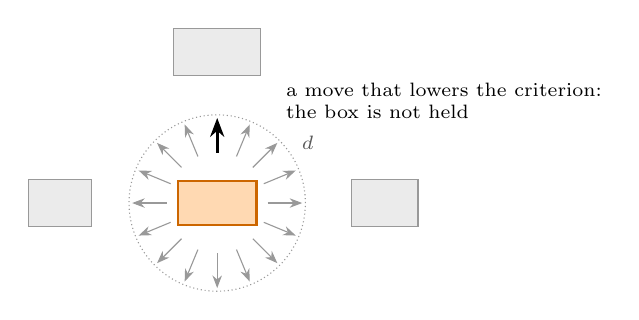
\begin{tikzpicture}[x=1cm,y=1cm,line width=0.4pt,font=\footnotesize]
  \draw[fill=black!8,draw=black!40] (-0.55,1.62) rectangle (0.55,2.22);
  \draw[fill=black!8,draw=black!40] (1.70,-0.30) rectangle (2.55,0.30);
  \draw[fill=black!8,draw=black!40] (-2.40,-0.30) rectangle (-1.60,0.30);
  \draw[densely dotted,black!40] (0,0) circle (1.12);
  \foreach \a in {0,22.5,45,67.5,112.5,135,157.5,180,202.5,225,247.5,270,292.5,315,337.5}{
    \draw[-{Stealth[length=1.6mm]},black!40] (\a:0.64) -- (\a:1.08);}
  \draw[-{Stealth[length=2.4mm]},black,line width=1pt] (90:0.64) -- (90:1.08);
  \draw[fill=orange!30,draw=orange!80!black,line width=0.8pt]
       (-0.5,-0.28) rectangle (0.5,0.28);
  \node[font=\scriptsize,black!65] at (33.75:1.38) {$d$};
  \node[anchor=west,font=\scriptsize,align=left] at (0.75,1.30)
       {a move that lowers the criterion:\\the box is not held};
\end{tikzpicture}
\caption{The test, one box and one criterion. The box is moved a distance $d$, two per
cent of the drawing's width, in each of sixteen exact directions, and the criterion is
recomputed. If some move lowers it (the dark arrow), the box is not held; if every move
raises it, the box is \emph{held}.}
\label{fig:test}
\end{figure}


\begin{center}\footnotesize
\begin{tabular}{lp{8.2cm}l}
\toprule
term & definition & zero when \\
\midrule
$T_C$ crossings & proper crossings between segments of two routes with no shared endpoint, $/m$ & planar \\
$T_O$ overlap & overlap area of boxes $/$ total box area & no overlap \\
$T_L$ length uniformity & mean over edges of $((\ell - L)/L)^2$ & all edges of length $L$ \\
$T_R$ orthogonality & mean over edges of the length-weighted mean over its segments of $\min(|\Delta x|,|\Delta y|)/(|\Delta x|+|\Delta y|)$ & routes axis-aligned \\
$T_A$ alignment & $1 -$ fraction of nodes in an alignment of $\ge 3$ (tol.\ 0.005) & every node aligned \\
$T_N$ node--edge & squared shortfall of node to foreign route distance below $(w+h)/4$ & none within \\
$T_F$ flow & mean over directed edges of the backward component along the reading direction $u$, over length & no edge runs back \\
\bottomrule
\end{tabular}
\end{center}

\section{The sums under composite energies}\label{app:sums}

At the hand layout the three base terms share the energy as length 0.99, crossings
0.01, overlap 0.00, and $C+O+L$ inherits the length term's zero.

\begin{center}\scriptsize\setlength{\tabcolsep}{3.5pt}
\begin{tabular}{llrrrrr}
\toprule
corpus & energy & hand & \texttt{neato} & \texttt{prism} & \texttt{dot} & \texttt{elk} \\
\midrule
WikiPathways & C$+$O & 1.00 [1.00, 1.00] & 0.60 & 1.00 & 1.00 & 1.00 \\
& C$+$O$+$L & 0.00 [0.00, 0.00] & 0.17 & 0.19 & 0.00 & 0.00 \\
& C$+$O$+$S & 0.00 [0.00, 0.00] & 0.60 & 0.94 & 0.00 & 0.00 \\
& C$+$O$+$R & 0.21 [0.19, 0.23] & 0.00 & 0.00 & 0.19 & 0.22 \\
& C$+$O$+$A1 & 0.51 [0.47, 0.53] & 0.04 & 0.07 & 1.00 & 0.57 \\
& C$+$O$+$A3 & 0.24 [0.22, 0.27] & 0.03 & 0.03 & 0.50 & 0.41 \\
& C$+$O$+$grid & 0.84 [0.81, 0.87] & 0.45 & 0.79 & 0.96 & 0.74 \\
& C$+$O$+$N & 0.86 [0.83, 0.88] & 0.55 & 1.00 & 0.78 & 0.74 \\
& C$+$O$+$F & 0.56 [0.53, 0.59] & 0.30 & 0.50 & 1.00 & 1.00 \\
\midrule
Reactome & C$+$O & 1.00 [1.00, 1.00] & 0.76 & 1.00 & 1.00 & 1.00 \\
& C$+$O$+$L & 0.00 [0.00, 0.00] & 0.33 & 0.27 & 0.00 & 0.00 \\
& C$+$O$+$S & 0.00 [0.00, 0.00] & 0.76 & 0.89 & 0.00 & 0.00 \\
& C$+$O$+$R & 0.17 [0.16, 0.19] & 0.00 & 0.00 & 0.14 & 0.13 \\
& C$+$O$+$A1 & 0.22 [0.19, 0.25] & 0.05 & 0.07 & 1.00 & 0.43 \\
& C$+$O$+$A3 & 0.11 [0.09, 0.12] & 0.03 & 0.03 & 0.42 & 0.33 \\
& C$+$O$+$grid & 0.64 [0.61, 0.67] & 0.52 & 0.75 & 0.94 & 0.73 \\
& C$+$O$+$N & 0.94 [0.91, 0.95] & 0.71 & 1.00 & 0.80 & 0.75 \\
& C$+$O$+$F & 0.61 [0.58, 0.65] & 0.33 & 0.44 & 1.00 & 1.00 \\
\midrule
BPMN & C$+$O & 1.00 [1.00, 1.00] & 0.41 & 1.00 & 1.00 & 1.00 \\
& C$+$O$+$L & 0.00 [0.00, 0.00] & 0.24 & 0.29 & 0.00 & 0.00 \\
& C$+$O$+$S & 0.00 [0.00, 0.00] & 0.43 & 0.92 & 0.00 & 0.00 \\
& C$+$O$+$R & 0.73 [0.71, 0.75] & 0.00 & 0.00 & 0.28 & 0.40 \\
& C$+$O$+$A1 & 0.89 [0.86, 0.95] & 0.04 & 0.09 & 0.88 & 0.68 \\
& C$+$O$+$A3 & 0.33 [0.30, 0.37] & 0.03 & 0.03 & 0.33 & 0.45 \\
& C$+$O$+$grid & 0.95 [0.93, 0.96] & 0.28 & 0.78 & 0.75 & 0.67 \\
& C$+$O$+$N & 1.00 [1.00, 1.00] & 0.40 & 1.00 & 0.82 & 0.76 \\
& C$+$O$+$F & 0.84 [0.81, 0.87] & 0.26 & 0.61 & 1.00 & 1.00 \\
\bottomrule
\end{tabular}
\end{center}

\begin{figure}[t]\centering
\begin{tabular}{@{}c@{\hspace{3pt}}c@{\hspace{3pt}}c@{\hspace{3pt}}c@{}}
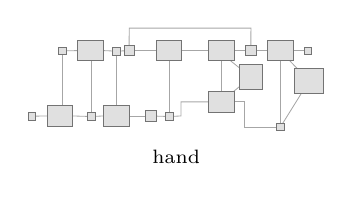
\begin{tikzpicture}[x=1cm,y=1cm,line width=0.3pt]
\draw[gray!70] (0.439,1.016) -- (0.632,1.019);
\draw[gray!70] (0.439,0.319) -- (0.439,1.016);
\draw[gray!70] (2.686,0.798) -- (2.572,0.889);
\draw[gray!70] (1.950,1.019) -- (2.292,1.019);
\draw[gray!70] (2.617,1.019) -- (2.829,1.019);
\draw[gray!70] (2.454,0.498) -- (2.454,0.889);
\draw[gray!70] (2.607,0.498) -- (2.686,0.563);
\draw[gray!70] (1.283,1.019) -- (1.624,1.019);
\draw[gray!70] (2.829,1.019) -- (2.830,1.305) -- (1.284,1.305) -- (1.283,1.019);
\draw[gray!70] (1.126,1.012) -- (1.283,1.019);
\draw[gray!70] (1.794,0.889) -- (1.794,0.182);
\draw[gray!70] (2.829,1.019) -- (3.040,1.019);
\draw[gray!70] (3.366,1.019) -- (3.558,1.019);
\draw[gray!70] (3.324,0.889) -- (3.418,0.791);
\draw[gray!70] (3.203,0.889) -- (3.203,0.046);
\draw[gray!70] (3.470,0.475) -- (3.203,0.046);
\draw[gray!70] (0.957,1.019) -- (1.126,1.012);
\draw[gray!70] (0.801,0.889) -- (0.801,0.182);
\draw[gray!70] (1.126,0.319) -- (1.126,1.012);
\draw[gray!70] (0.049,0.186) -- (0.241,0.189);
\draw[gray!70] (0.566,0.189) -- (0.801,0.182);
\draw[gray!70] (0.801,0.182) -- (0.957,0.189);
\draw[gray!70] (1.283,0.189) -- (1.559,0.189);
\draw[gray!70] (1.794,0.182) -- (1.942,0.189) -- (1.942,0.368) -- (2.292,0.368);
\draw[gray!70] (1.559,0.189) -- (1.794,0.182);
\draw[gray!70] (2.617,0.368) -- (2.744,0.368) -- (2.744,0.046) -- (3.203,0.046);
\draw[fill=black!12,draw=black!55] (0.391,0.967) rectangle (0.488,1.064);
\draw[fill=black!12,draw=black!55] (2.292,0.889) rectangle (2.617,1.149);
\draw[fill=black!12,draw=black!55] (2.686,0.524) rectangle (2.972,0.840);
\draw[fill=black!12,draw=black!55] (1.217,0.954) rectangle (1.348,1.084);
\draw[fill=black!12,draw=black!55] (1.624,0.889) rectangle (1.950,1.149);
\draw[fill=black!12,draw=black!55] (2.764,0.954) rectangle (2.894,1.084);
\draw[fill=black!12,draw=black!55] (3.040,0.889) rectangle (3.366,1.149);
\draw[fill=black!12,draw=black!55] (3.512,0.973) rectangle (3.604,1.064);
\draw[fill=black!12,draw=black!55] (3.385,0.475) rectangle (3.750,0.791);
\draw[fill=black!12,draw=black!55] (0.632,0.889) rectangle (0.957,1.149);
\draw[fill=black!12,draw=black!55] (1.077,0.964) rectangle (1.175,1.061);
\draw[fill=black!12,draw=black!55] (0.000,0.137) rectangle (0.098,0.234);
\draw[fill=black!12,draw=black!55] (0.241,0.059) rectangle (0.566,0.319);
\draw[fill=black!12,draw=black!55] (0.752,0.133) rectangle (0.850,0.231);
\draw[fill=black!12,draw=black!55] (0.957,0.059) rectangle (1.283,0.319);
\draw[fill=black!12,draw=black!55] (1.745,0.133) rectangle (1.842,0.231);
\draw[fill=black!12,draw=black!55] (2.292,0.238) rectangle (2.617,0.498);
\draw[fill=black!12,draw=black!55] (1.494,0.124) rectangle (1.624,0.254);
\draw[fill=black!12,draw=black!55] (3.158,0.000) rectangle (3.249,0.091);
\node[anchor=north,font=\scriptsize] at (1.88,-0.12) {hand};
\end{tikzpicture}
&
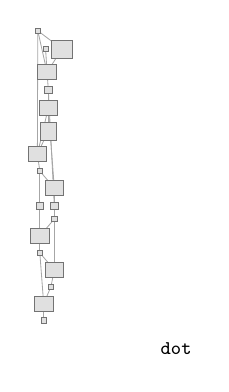
\begin{tikzpicture}[x=1cm,y=1cm,line width=0.3pt]
\draw[gray!70] (0.290,0.465) -- (0.333,0.680);
\draw[gray!70] (0.198,0.250) -- (0.290,0.465);
\draw[gray!70] (0.257,2.443) -- (0.257,2.737);
\draw[gray!70] (0.333,1.719) -- (0.257,2.737);
\draw[gray!70] (0.257,2.737) -- (0.257,2.964);
\draw[gray!70] (0.118,2.149) -- (0.257,2.737);
\draw[gray!70] (0.118,2.149) -- (0.257,2.443);
\draw[gray!70] (0.333,1.492) -- (0.333,1.719);
\draw[gray!70] (0.257,2.964) -- (0.333,1.492);
\draw[gray!70] (0.333,1.325) -- (0.333,1.492);
\draw[gray!70] (0.333,1.719) -- (0.149,1.934);
\draw[gray!70] (0.257,2.964) -- (0.241,3.190);
\draw[gray!70] (0.241,3.190) -- (0.222,3.484);
\draw[gray!70] (0.241,3.190) -- (0.430,3.484);
\draw[gray!70] (0.241,3.190) -- (0.123,3.717);
\draw[gray!70] (0.430,3.484) -- (0.123,3.717);
\draw[gray!70] (0.333,0.680) -- (0.333,1.325);
\draw[gray!70] (0.333,0.680) -- (0.149,0.895);
\draw[gray!70] (0.149,1.110) -- (0.333,1.325);
\draw[gray!70] (0.198,0.035) -- (0.198,0.250);
\draw[gray!70] (0.198,0.250) -- (0.149,0.895);
\draw[gray!70] (0.149,0.895) -- (0.149,1.110);
\draw[gray!70] (0.149,1.110) -- (0.149,1.492);
\draw[gray!70] (0.149,1.934) -- (0.118,2.149);
\draw[gray!70] (0.149,1.492) -- (0.149,1.934);
\draw[gray!70] (0.118,2.149) -- (0.123,3.717);
\draw[fill=black!12,draw=black!55] (0.255,0.430) rectangle (0.326,0.501);
\draw[fill=black!12,draw=black!55] (0.139,2.642) rectangle (0.375,2.831);
\draw[fill=black!12,draw=black!55] (0.154,2.328) rectangle (0.361,2.557);
\draw[fill=black!12,draw=black!55] (0.286,1.445) rectangle (0.380,1.540);
\draw[fill=black!12,draw=black!55] (0.215,1.625) rectangle (0.451,1.814);
\draw[fill=black!12,draw=black!55] (0.210,2.916) rectangle (0.305,3.011);
\draw[fill=black!12,draw=black!55] (0.123,3.096) rectangle (0.359,3.285);
\draw[fill=black!12,draw=black!55] (0.189,3.451) rectangle (0.255,3.517);
\draw[fill=black!12,draw=black!55] (0.298,3.370) rectangle (0.562,3.599);
\draw[fill=black!12,draw=black!55] (0.215,0.586) rectangle (0.451,0.774);
\draw[fill=black!12,draw=black!55] (0.298,1.289) rectangle (0.368,1.360);
\draw[fill=black!12,draw=black!55] (0.163,0.000) rectangle (0.234,0.071);
\draw[fill=black!12,draw=black!55] (0.080,0.156) rectangle (0.316,0.345);
\draw[fill=black!12,draw=black!55] (0.113,0.859) rectangle (0.184,0.930);
\draw[fill=black!12,draw=black!55] (0.031,1.015) rectangle (0.267,1.204);
\draw[fill=black!12,draw=black!55] (0.113,1.899) rectangle (0.184,1.969);
\draw[fill=black!12,draw=black!55] (0.000,2.054) rectangle (0.236,2.243);
\draw[fill=black!12,draw=black!55] (0.102,1.445) rectangle (0.196,1.540);
\draw[fill=black!12,draw=black!55] (0.090,3.684) rectangle (0.156,3.750);
\node[anchor=north,font=\scriptsize] at (1.88,-0.12) {\texttt{dot}};
\end{tikzpicture}
&
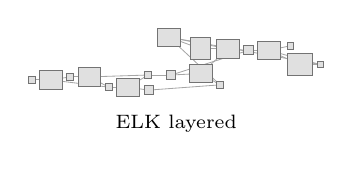
\begin{tikzpicture}[x=1cm,y=1cm,line width=0.3pt]
\draw[gray!70] (0.534,0.245) -- (0.779,0.245);
\draw[gray!70] (0.288,0.207) -- (0.534,0.245);
\draw[gray!70] (2.192,0.601) -- (2.538,0.601);
\draw[gray!70] (2.192,0.288) -- (2.538,0.601);
\draw[gray!70] (2.538,0.601) -- (2.798,0.582);
\draw[gray!70] (1.788,0.750) -- (2.538,0.601);
\draw[gray!70] (1.788,0.750) -- (2.192,0.601);
\draw[gray!70] (1.817,0.269) -- (2.192,0.288);
\draw[gray!70] (2.798,0.582) -- (1.817,0.269);
\draw[gray!70] (1.524,0.269) -- (1.817,0.269);
\draw[gray!70] (2.192,0.288) -- (2.438,0.144);
\draw[gray!70] (2.798,0.582) -- (3.058,0.582);
\draw[gray!70] (3.058,0.582) -- (3.329,0.640);
\draw[gray!70] (3.058,0.582) -- (3.450,0.402);
\draw[gray!70] (3.058,0.582) -- (3.710,0.402);
\draw[gray!70] (3.450,0.402) -- (3.710,0.402);
\draw[gray!70] (0.779,0.245) -- (1.524,0.269);
\draw[gray!70] (0.779,0.245) -- (1.024,0.115);
\draw[gray!70] (1.269,0.115) -- (1.524,0.269);
\draw[gray!70] (0.043,0.207) -- (0.288,0.207);
\draw[gray!70] (0.288,0.207) -- (1.024,0.115);
\draw[gray!70] (1.024,0.115) -- (1.269,0.115);
\draw[gray!70] (1.269,0.115) -- (1.529,0.077);
\draw[gray!70] (2.438,0.144) -- (1.788,0.750);
\draw[gray!70] (1.529,0.077) -- (2.438,0.144);
\draw[gray!70] (1.788,0.750) -- (3.710,0.402);
\draw[fill=black!12,draw=black!55] (0.490,0.202) rectangle (0.577,0.288);
\draw[fill=black!12,draw=black!55] (2.394,0.486) rectangle (2.683,0.717);
\draw[fill=black!12,draw=black!55] (2.065,0.462) rectangle (2.319,0.741);
\draw[fill=black!12,draw=black!55] (1.760,0.212) rectangle (1.875,0.327);
\draw[fill=black!12,draw=black!55] (2.048,0.173) rectangle (2.337,0.404);
\draw[fill=black!12,draw=black!55] (2.740,0.525) rectangle (2.856,0.640);
\draw[fill=black!12,draw=black!55] (2.913,0.467) rectangle (3.202,0.698);
\draw[fill=black!12,draw=black!55] (3.288,0.600) rectangle (3.369,0.680);
\draw[fill=black!12,draw=black!55] (3.288,0.262) rectangle (3.612,0.542);
\draw[fill=black!12,draw=black!55] (0.635,0.130) rectangle (0.923,0.361);
\draw[fill=black!12,draw=black!55] (1.481,0.226) rectangle (1.567,0.312);
\draw[fill=black!12,draw=black!55] (0.000,0.163) rectangle (0.087,0.250);
\draw[fill=black!12,draw=black!55] (0.144,0.091) rectangle (0.433,0.322);
\draw[fill=black!12,draw=black!55] (0.981,0.072) rectangle (1.067,0.159);
\draw[fill=black!12,draw=black!55] (1.125,0.000) rectangle (1.413,0.231);
\draw[fill=black!12,draw=black!55] (2.394,0.101) rectangle (2.481,0.188);
\draw[fill=black!12,draw=black!55] (1.644,0.635) rectangle (1.933,0.865);
\draw[fill=black!12,draw=black!55] (1.471,0.019) rectangle (1.587,0.135);
\draw[fill=black!12,draw=black!55] (3.669,0.362) rectangle (3.750,0.442);
\node[anchor=north,font=\scriptsize] at (1.88,-0.12) {ELK layered};
\end{tikzpicture}
&
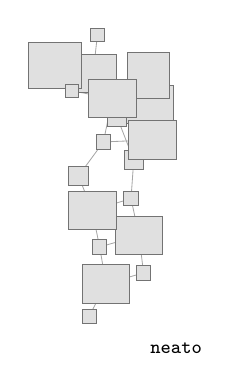
\begin{tikzpicture}[x=1cm,y=1cm,line width=0.3pt]
\draw[gray!70] (1.466,0.642) -- (1.409,1.115);
\draw[gray!70] (0.989,0.501) -- (1.466,0.642);
\draw[gray!70] (1.528,3.147) -- (1.542,2.781);
\draw[gray!70] (1.579,2.330) -- (1.542,2.781);
\draw[gray!70] (1.542,2.781) -- (1.130,2.620);
\draw[gray!70] (1.069,2.855) -- (1.542,2.781);
\draw[gray!70] (1.069,2.855) -- (1.528,3.147);
\draw[gray!70] (1.342,2.074) -- (1.579,2.330);
\draw[gray!70] (1.130,2.620) -- (1.342,2.074);
\draw[gray!70] (1.307,1.584) -- (1.342,2.074);
\draw[gray!70] (1.579,2.330) -- (0.957,2.304);
\draw[gray!70] (1.130,2.620) -- (0.825,3.170);
\draw[gray!70] (0.825,3.170) -- (0.881,3.665);
\draw[gray!70] (0.825,3.170) -- (0.339,3.274);
\draw[gray!70] (0.825,3.170) -- (0.555,2.954);
\draw[gray!70] (0.339,3.274) -- (0.555,2.954);
\draw[gray!70] (1.409,1.115) -- (1.307,1.584);
\draw[gray!70] (1.409,1.115) -- (0.909,0.970);
\draw[gray!70] (0.813,1.436) -- (1.307,1.584);
\draw[gray!70] (0.776,0.091) -- (0.989,0.501);
\draw[gray!70] (0.989,0.501) -- (0.909,0.970);
\draw[gray!70] (0.909,0.970) -- (0.813,1.436);
\draw[gray!70] (0.813,1.436) -- (0.640,1.872);
\draw[gray!70] (0.957,2.304) -- (1.069,2.855);
\draw[gray!70] (0.640,1.872) -- (0.957,2.304);
\draw[gray!70] (1.069,2.855) -- (0.555,2.954);
\draw[fill=black!12,draw=black!55] (1.375,0.551) rectangle (1.557,0.733);
\draw[fill=black!12,draw=black!55] (1.239,2.539) rectangle (1.845,3.024);
\draw[fill=black!12,draw=black!55] (1.262,2.853) rectangle (1.795,3.441);
\draw[fill=black!12,draw=black!55] (1.220,1.953) rectangle (1.463,2.195);
\draw[fill=black!12,draw=black!55] (1.276,2.087) rectangle (1.882,2.572);
\draw[fill=black!12,draw=black!55] (1.009,2.499) rectangle (1.251,2.741);
\draw[fill=black!12,draw=black!55] (0.522,2.927) rectangle (1.128,3.412);
\draw[fill=black!12,draw=black!55] (0.796,3.580) rectangle (0.966,3.750);
\draw[fill=black!12,draw=black!55] (0.000,2.980) rectangle (0.679,3.568);
\draw[fill=black!12,draw=black!55] (1.106,0.873) rectangle (1.712,1.358);
\draw[fill=black!12,draw=black!55] (1.216,1.493) rectangle (1.398,1.675);
\draw[fill=black!12,draw=black!55] (0.685,0.000) rectangle (0.867,0.182);
\draw[fill=black!12,draw=black!55] (0.686,0.259) rectangle (1.292,0.744);
\draw[fill=black!12,draw=black!55] (0.818,0.879) rectangle (1.000,1.061);
\draw[fill=black!12,draw=black!55] (0.510,1.193) rectangle (1.116,1.678);
\draw[fill=black!12,draw=black!55] (0.866,2.213) rectangle (1.048,2.395);
\draw[fill=black!12,draw=black!55] (0.766,2.612) rectangle (1.372,3.097);
\draw[fill=black!12,draw=black!55] (0.518,1.751) rectangle (0.761,1.994);
\draw[fill=black!12,draw=black!55] (0.470,2.870) rectangle (0.640,3.039);
\node[anchor=north,font=\scriptsize] at (1.88,-0.12) {\texttt{neato}};
\end{tikzpicture}
\end{tabular}
\caption{The same graph, the same box sizes, four layouts. The hand drawing and the two
layered tools share the profile the test reads: held under overlap, free under length and
stress. \texttt{neato} minimises stress and is the control that gives the test its power,
held at 1.00 under stress where every hand layout reads 0.00. The tool layouts carry no
waypoints, so their edges are drawn as chords.}
\label{fig:tools}
\end{figure}


\section{Decrease and active, term by term}\label{app:flat}

The gridiness value puts 58\%, 36\% and 82\% of hand-placed
boxes in an alignment of three or more, none of \texttt{neato}'s, 88\%, 82\% and 78\% of
\texttt{dot}'s and 80\%, 69\% and 75\% of ELK's. The gridiness $q$ of 0.77 to 0.78 on \texttt{neato}'s layouts, at value
1.000, is the step term's flatness, so alignment is compared on the value.
Node--edge separation is nearly satisfied in every layout (0.000 to 0.021) and holds 0.74
to 1.00 for the same reason. Crossings hold every box at this radius; the median value on
the routes is 0.000 by hand in every corpus and 0.000 for \texttt{neato}, 0.029, 0.056 and
0.000 for \texttt{dot}, 0.036, 0.066 and 0.000 for ELK. Under flow \texttt{dot} and ELK
are held at 1.00 with the term at 0.000 in every corpus; the hand layouts hold 0.59, 0.62
and 0.85 at 0.131, 0.096 and 0.045, and \texttt{neato}, which knows no direction, 0.44 to
0.62 at 0.121 to 0.222.

\paragraph{Step terms.} A count (crossings) or a step function of position (gridiness,
Section~\ref{sec:method}) is flat almost everywhere and holds a node wherever no move of
length $d$ changes it. There $q_d$ measures how much of the layout the criterion has stopped
acting on, not how well it is met, so the term's value is reported beside $q_d$.

An interval of [0.00, 0.00] or [1.00, 1.00] is a pileup at the boundary, not precision: 87 to 92\% of hand diagrams sit at exactly 0.00 under length and stress, and 62 to 85\% of \texttt{neato}'s at exactly 1.00 under stress (\texttt{results/robustness.md}).

\paragraph{What $q$ counts, term by term.} A held fraction is not commensurable across
terms of different shape, and reading down a column compares three different things. Beside
each $q$ the table gives \emph{dec}, the median over diagrams of the per-diagram mean best
decrease a single move finds as a fraction of the term's value, and \emph{active}, the share of diagrams in which
any box has an improving move at all. Where \emph{active} is small the term is flat at this
radius: it holds every box without being satisfied by any of them, and its 1.00 carries no
information about the person.

\begin{center}\small
\begin{tabular}{@{}lccc@{\hspace{14pt}}ccc@{\hspace{14pt}}ccc@{}}
\toprule
& \multicolumn{3}{c}{WikiPathways} & \multicolumn{3}{c}{Reactome} & \multicolumn{3}{c}{BPMN} \\
\cmidrule(r){2-4}\cmidrule(r){5-7}\cmidrule{8-10}
term & $q$ & dec & active & $q$ & dec & active & $q$ & dec & active \\
\midrule
crossings      & 1.00 & 0.000 & 30\% & 1.00 & 0.000 & 20\% & 1.00 & 0.000 & 3\% \\
overlap        & 1.00 & 0.000 & 18\% & 1.00 & 0.000 & 4\%  & 1.00 & 0.000 & 7\% \\
node--edge     & 0.88 & 0.047 & 64\% & 1.00 & 0.000 & 49\% & 1.00 & 0.000 & 15\% \\
\midrule
length         & 0.00 & 0.013 & 100\% & 0.00 & 0.013 & 100\% & 0.00 & 0.012 & 100\% \\
stress         & 0.00 & 0.005 & 100\% & 0.00 & 0.006 & 100\% & 0.00 & 0.007 & 100\% \\
orthogonality  & 0.19 & 0.012 & 100\% & 0.17 & 0.027 & 100\% & 0.72 & 0.008 & 99\% \\
alignment A1   & 0.52 & 0.066 & 92\%  & 0.21 & 0.069 & 99\%  & 0.91 & 0.032 & 56\% \\
flow           & 0.59 & 0.010 & 90\%  & 0.62 & 0.012 & 95\%  & 0.85 & 0.005 & 74\% \\
\bottomrule
\end{tabular}
\end{center}

\section{Sensitivities}\label{app:sens}

The attachment point matters: of the 2{,}584 BPMN routes that carry an interior
waypoint, 0.27 are axis-aligned at every segment when the route is closed at the box
centres and 0.88 when it is closed at the stored attachments.

This is not a new device. Minimising a stress term
over a scale factor is Smelser, Miller and Kobourov's scale-normalised stress
\cite{smelser24}, who give the minimiser in closed form and read it as a correlation
coefficient, and Ahmed et al.\ \cite{ahmed24} derive the same for the $\delta_{ij}$-weighted
graph stress used here. Their result is also why the fixed-$L$ reading above is not a
curiosity: under scale-sensitive stress they find a random layout ranked ahead of both
\texttt{neato} and SFDP on nearly every graph of two 1{,}000-graph benchmarks. A
control that reads $0.07$ at a fixed $L$ is that pathology, and fitting $L$ is the known
repair.

\paragraph{Radius.} $q_d$ at $d \in \{0.005, 0.01, 0.02, 0.05\}$, hand layouts, then
\texttt{neato}'s (\texttt{profile.py --sweep}):

\begin{center}\footnotesize
\begin{tabular}{lrrrrrrrrrrrr}
\toprule
 & \multicolumn{4}{c}{WikiPathways} & \multicolumn{4}{c}{Reactome} & \multicolumn{4}{c}{BPMN} \\
energy & .005 & .01 & .02 & .05 & .005 & .01 & .02 & .05 & .005 & .01 & .02 & .05 \\
\midrule
overlap, hand & 1.00 & 1.00 & 1.00 & 1.00 & 1.00 & 1.00 & 1.00 & 1.00 & 1.00 & 1.00 & 1.00 & 1.00 \\
length, hand & 0.00 & 0.00 & 0.00 & 0.00 & 0.00 & 0.00 & 0.00 & 0.00 & 0.00 & 0.00 & 0.00 & 0.00 \\
stress, hand & 0.00 & 0.00 & 0.00 & 0.00 & 0.00 & 0.00 & 0.00 & 0.00 & 0.00 & 0.00 & 0.00 & 0.00 \\
alignment A1, hand & 0.52 & 0.54 & 0.52 & 0.44 & 0.12 & 0.17 & 0.21 & 0.19 & 0.90 & 0.91 & 0.91 & 0.87 \\
gridiness, hand & 0.94 & 0.91 & 0.87 & 0.75 & 0.82 & 0.75 & 0.65 & 0.57 & 1.00 & 1.00 & 0.95 & 0.88 \\
flow, hand & 0.59 & 0.59 & 0.59 & 0.59 & 0.62 & 0.62 & 0.62 & 0.63 & 0.85 & 0.85 & 0.85 & 0.85 \\
\midrule
overlap, \texttt{neato} & 0.60 & 0.60 & 0.60 & 0.60 & 0.75 & 0.76 & 0.76 & 0.76 & 0.41 & 0.41 & 0.41 & 0.43 \\
length, \texttt{neato} & 0.04 & 0.12 & 0.24 & 0.47 & 0.07 & 0.19 & 0.35 & 0.58 & 0.08 & 0.22 & 0.42 & 0.72 \\
stress, \texttt{neato} & 0.90 & 0.96 & 1.00 & 1.00 & 0.96 & 1.00 & 1.00 & 1.00 & 0.94 & 0.97 & 1.00 & 1.00 \\
alignment A1, \texttt{neato} & 0.04 & 0.05 & 0.06 & 0.06 & 0.03 & 0.05 & 0.06 & 0.07 & 0.03 & 0.05 & 0.06 & 0.07 \\
gridiness, \texttt{neato} & 0.93 & 0.86 & 0.78 & 0.65 & 0.90 & 0.83 & 0.77 & 0.61 & 0.92 & 0.85 & 0.78 & 0.67 \\
flow, \texttt{neato} & 0.50 & 0.50 & 0.50 & 0.50 & 0.45 & 0.45 & 0.45 & 0.45 & 0.62 & 0.62 & 0.62 & 0.62 \\
\bottomrule
\end{tabular}
\end{center}

The hand verdicts do not move with the radius. \texttt{neato}'s under length do: a smooth
term near a minimum with gradient $g$ and curvature $\lambda$ holds a node when
$|g| < d\lambda/2$, so a layout that is nearly a minimum is held at a large radius and
free at a small one, and \texttt{neato}'s layouts, which minimise stress and not length
uniformity, read as nearly uniform at $d = 0.05$ (0.47 to 0.70) and not at $d = 0.005$
(0.04 to 0.08). A hand layout at 0.00 across the range is far from the minimum at every
scale the test resolves. Gridiness falls with $d$ in every layout because a larger move
reaches an alignment from further away; flow, a projection, does not move with $d$ at all.
ELK's block (\texttt{results/sweep.md}) reads as \texttt{dot}'s: length and stress 0.00 at
every radius, flow 1.00 at every radius.

\paragraph{Directions.} Each doubling of $V$ contains the previous set, so $q$ can only
fall as directions are added and the primary sixteen-direction figures are upper bounds on
the continuum value (\texttt{results/robustness.md}). At 8, 16, 32 and 64 directions the
verdicts stand: hand length and stress 0.00 in every corpus at every count,
\texttt{neato}'s stress 1.00 at every count. The alignment level is what moves: A1 by hand
reads 0.58, 0.52, 0.47, 0.39 on WikiPathways, 0.31, 0.21, 0.14, 0.07 on Reactome and 0.92,
0.91, 0.90, 0.86 on BPMN across the four counts, while \texttt{neato}'s 0.06 falls to
0.00. The hand-to-control gap survives at 64; the levels are comparable only at one count
and are stated at sixteen. The full grid of radius, direction count, reference-length
rule and route treatment, 1{,}008 cells, flips no verdict: under the fitted $L$ the hand
distance terms read exactly 0.00 in every cell (\texttt{results/specgrid.md}). The tie
tolerance, the last instrument constant, moves nothing at all: the A1 medians are
identical at 0.001 through 0.01 (\texttt{results/tolsweep.md}), so the alignments the
test counts are exact ties, not tolerance-window artefacts.

\paragraph{Reference length.} Under the median edge length instead of the fitted $L$,
\texttt{neato}'s stress layouts score 0.07, 0.08 and 0.12 under stress and the hand
layouts 0.00; under length the hand layouts score 0.03, 0.04 and 0.05 and \texttt{neato}'s
0.26, 0.41 and 0.45. Under $L = 1/\sqrt{N}$ no box of any layout is held under either term,
the scale being wrong for every layout. The hand verdicts do not depend on the choice; the
control's does, so the fit is primary (Section~\ref{sec:foundations}).

\paragraph{Box extent.} Centre distances on box diagrams could be the objection: with
large, uneven boxes a person could sit at a minimum of a border-to-border distance term
while failing the centre one. Measured border to border, each box's offset to its border
along the joining direction subtracted and $L$ refitted on those distances, the hand
verdicts do not move: length and stress hold 0.00 in every corpus, 0.86 to 0.92 of
diagrams at exactly zero (\texttt{results/border.py}). \texttt{neato}, which minimised
the centre form, is not held under the border form (0.00 to 0.09), as a layout optimising
one criterion and tested on another should not be.





\paragraph{Routes.} The tables of Section~\ref{sec:results} are on the stored routes; the chords are the
sensitivity, \texttt{chords.md} beside the tables in the repository. Closing every edge at the box centres moves no
verdict: crossings still hold every box (the WikiPathways value rises from 0.000 to 0.038,
one crossing per 26 edges, the anchors' work), orthogonality falls from 0.19, 0.17 and
0.73 to 0.16, 0.05 and 0.40, and node--edge separation from 0.88, 1.00 and 1.00 to 0.76,
0.85 and 0.87. The drawn geometry only raises the hand layout's standing on the criteria
it touches.

Each format's stored routes, as a fraction of the edges in the band:

\begin{center}\scriptsize
\begin{tabular}{lrrl}
\toprule
corpus & edges & with a waypoint & by what the file stores \\
\midrule
WikiPathways & 8{,}253 & 0.291 & chord 0.587, anchor 0.225, elbow 0.154, curved 0.026, segmented 0.008 \\
Reactome & 6{,}827 & 0.069 & chord 0.931, stored 0.069 \\
BPMN & 7{,}910 & 0.327 & chord 0.673, stored 0.327 \\
\bottomrule
\end{tabular}
\end{center}

GPML's Elbow and Curved connectors store
their endpoints only and PathVisio computes the bends at draw time, so those routes read as
chords; a quarter of WikiPathways edges end on an anchor of another interaction, where the
person drew no segment to the node and the last segment is manufactured. Only the BPMN
routes are orthogonal: of the WikiPathways and Reactome routes with a waypoint, 0.009 and
0.007 are axis-aligned at every segment, the biological formats drawing diagonal segments.
The chords are the sensitivity.

\begin{figure}[t]\centering
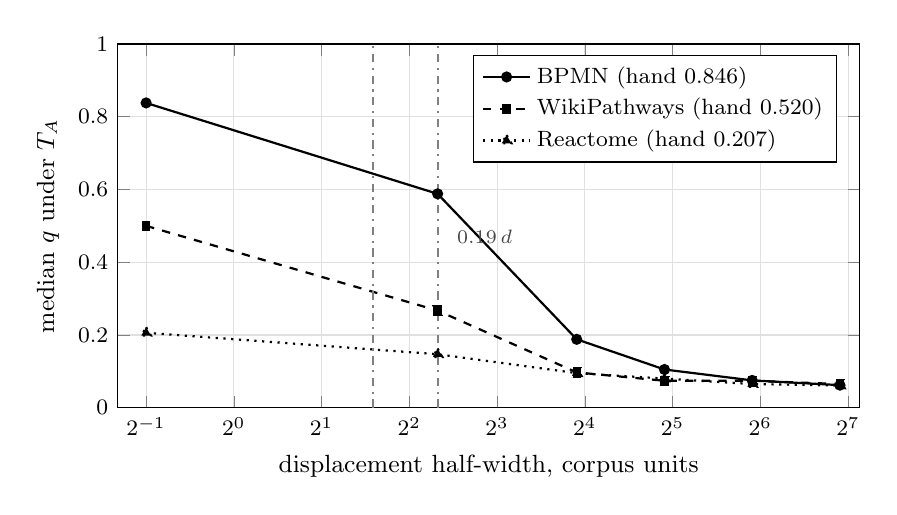
\begin{tikzpicture}
\begin{axis}[width=11cm,height=6.2cm,
  xmode=log,log basis x=2,
  xlabel={displacement half-width, corpus units},
  ylabel={median $q$ under $T_A$},
  ymin=0,ymax=1,xmin=0.4,xmax=140,
  legend pos=north east,legend cell align=left,
  grid=major,grid style={black!12},
  tick label style={font=\footnotesize},label style={font=\small},
  legend style={font=\footnotesize}]
\addplot[thick,mark=*,mark size=1.6pt] coordinates
  {(0.5,0.838)(5,0.588)(15,0.188)(30,0.105)(60,0.075)(120,0.062)};
\addlegendentry{BPMN (hand 0.846)}
\addplot[thick,mark=square*,mark size=1.5pt,dashed] coordinates
  {(0.5,0.500)(5,0.267)(15,0.097)(30,0.074)(60,0.074)(120,0.065)};
\addlegendentry{WikiPathways (hand 0.520)}
\addplot[thick,mark=triangle*,mark size=2pt,dotted] coordinates
  {(0.5,0.206)(5,0.147)(15,0.095)(30,0.080)(60,0.065)(120,0.061)};
\addlegendentry{Reactome (hand 0.207)}
\addplot[gray,thick,dash dot,forget plot] coordinates {(3,0)(3,1)};
\addplot[gray,thick,dash dot,forget plot] coordinates {(5,0)(5,1)};
\node[anchor=west,font=\scriptsize,gray!55!black] at (axis cs:5.4,0.47) {$0.19\,d$};
\end{axis}
\end{tikzpicture}
\caption{The displacement sweep, every box of every hand layout displaced by up to the
half-width, the alignment hold read at $d = 0.02$ and sixteen directions. The declared
half-pitch test sits at the left edge, 0.5 units, where nothing has changed: the corner of
$T_A$ releases a box only past $0.19\,d$, 3 units in the biological corpora and 5 in
BPMN. Past the bound the hold falls, BPMN 0.84 to 0.59 by a half-width of 5, and by 120
units every corpus is at the grid-snapped level of 0.06 to 0.09.}
\label{fig:sweep}
\end{figure}


\section{Descent, chance and the displacement yardstick}\label{app:descent}

\paragraph{The descent, in full.} Through the library: hill climbing from the hand layout,
one node per proposal, first step $d/2$ per coordinate, the step halved after 200 rejected
proposals, each node kept within a disc of radius $d$ about its start by the repair, 4000
energy evaluations, 15 seeds per instance; and uniform sampling in the same cap at the same
budget on the same seeds, the matched-budget control. Reported per instance: the fraction
of the cap used (mean over nodes of the distance moved over $d$), the fraction of energy
removed, for the climber and for the control, and the number of seeds on which the climber
ends lower than the control with its exact sign test. The climber pilot used a step of
$0.1$, five times the cap, so that nearly every proposal landed on the cap circle; the base-energy result did not depend on it (98.5 to 95.9\% of the cap used as the step fell from 0.1 to 0.005) and the alignment result did (47 to 18\%), so the directional test is primary. The converged reference is the same climber uncapped, 60{,}000 evaluations, with $q_d$ measured where it stops.

\paragraph{Descent and chance.} The secondary estimand, per corpus and energy: the median
fraction of the cap the capped climber uses and of the energy it removes, the same for
uniform sampling in the cap at the same budget and seeds, the share of diagrams where the
climber ends lower on at least 12 of 15 seeds, and $q_{0.02}$ where the uncapped climber
stops, the converged reference.

\begin{center}\footnotesize
\begin{tabular}{llrrrrrr}
\toprule
 & & \multicolumn{2}{c}{cap used} & \multicolumn{2}{c}{energy removed} & & \\
corpus & energy & climb & random & climb & random & $\ge$12/15 & $q$ conv. \\
\midrule
WikiPathways & C$+$O$+$L & 0.99 & 0.76 & 0.28 & 0.16 & 0.88 & 1.00 \\
 & C$+$O$+$A1 & 0.39 & 0.74 & 0.71 & 0.17 & 0.75 & 1.00 \\
 & stress & 1.00 & 0.77 & 0.12 & 0.05 & 1.00 & 1.00 \\
 & C$+$O$+$F & 0.44 & 0.76 & 0.27 & 0.18 & 0.77 & 1.00 \\
\midrule
Reactome & C$+$O$+$L & 1.00 & 0.76 & 0.31 & 0.16 & 0.93 & 1.00 \\
 & C$+$O$+$A1 & 0.56 & 0.74 & 0.99 & 0.37 & 0.80 & 1.00 \\
 & stress & 1.00 & 0.77 & 0.13 & 0.06 & 1.00 & 1.00 \\
 & C$+$O$+$F & 0.36 & 0.75 & 0.32 & 0.22 & 0.71 & 1.00 \\
\midrule
BPMN & C$+$O$+$L & 1.00 & 0.77 & 0.26 & 0.12 & 0.99 & 1.00 \\
 & C$+$O$+$A1 & 0.11 & 0.73 & 0.24 & $-$0.01 & 0.95 & 1.00 \\
 & stress & 1.00 & 0.77 & 0.14 & 0.07 & 1.00 & 1.00 \\
 & C$+$O$+$F & 0.16 & 0.74 & 0.09 & 0.04 & 0.66 & 1.00 \\
\bottomrule
\end{tabular}
\end{center}

Under the distance energies the climber walks every node to the cap circle (0.99 to 1.00 of
$d$) and is still removing energy when the budget ends; under C$+$O$+$A1 it moves 0.11 to
0.56 of the cap, the misalignments being nearer than $d$. The climber beats the control on
all 15 seeds, which survives Holm over the corpus (exact sign $p = 3.1 \times 10^{-5}$
against $0.05/305$), on 0.81 to 0.99 of diagrams under C$+$O$+$L and on all of them under
stress. The converged reference's median $q$ is 1.00 for every energy and corpus, the
test's power on the sums; the fraction of diagrams whose reference stops below 0.9 is at
most 0.02 everywhere but C$+$O$+$F (0.05, 0.07 and 0.13), the flow term's plateaus.

\paragraph{The displacement yardstick.} Perturb \texttt{neato}'s converged stress
layouts, every box moved a known fraction of the width in a seeded direction, and run
the same capped climber (\texttt{results/calib.py}). Unperturbed it removes 0.001 of the
stress energy; at a displacement of 0.005, 0.007 to 0.024; at 0.02, 0.09 to 0.26; at
0.05, 0.24 to 0.43; at 0.10 less again, the cap seeing a shrinking share of a growing
energy. The hand layouts' 0.12 to 0.14 under stress sits at a displacement of 0.014 to
0.025.

\section{The paired tests in full}\label{app:pairs}

\paragraph{The statistics, in full.} The unit of inference is the diagram. Per corpus, the paired
comparison of $q_d$ between the hand layout and a tool control is the Wilcoxon signed-rank
test, zeros dropped, ties by midranks, exact on the observed ranks up to 50 non-zero pairs
and the normal approximation with continuity and tie corrections above, with the exact sign
test beside it and the Hodges--Lehmann shift with its distribution-free 95\% interval; the
family is the terms compared against one control within one corpus, Holm-corrected. The
script carries 630 self-checks against enumeration and against R. Equivalence claims (``no
reweighting repairs it'') are read off the sweep, never off a failure to reject.

The columns are those of Section~\ref{sec:results}: the Hodges--Lehmann shift of
$q_{0.02}$, hand against \texttt{dot}, with the Holm-adjusted signed-rank $p$.

\begin{center}\scriptsize
\begin{tabular}{lrrrrrr}
\toprule
 & \multicolumn{2}{c}{WikiPathways} & \multicolumn{2}{c}{Reactome} & \multicolumn{2}{c}{BPMN} \\
energy & HL [95\%] & $p$ & HL [95\%] & $p$ & HL [95\%] & $p$ \\
\midrule
crossings & $-0.04$ [$-0.07$, $-0.01$] & 0.016 & $+0.02$ [$-0.01$, $+0.05$] & 0.30 & $+0.10$ [$+0.08$, $+0.12$] & $<$1e-4 \\
overlap & $-0.14$ [$-0.18$, $-0.11$] & $<$1e-4 & $-0.07$ [$-0.10$, $-0.06$] & 0.0024 & $-0.22$ [$-0.29$, $-0.11$] & $<$1e-4 \\
length & $-0.01$ [$-0.03$, $+0.00$] & 0.27 & $-0.03$ [$-0.05$, $-0.01$] & 0.017 & $-0.09$ [$-0.12$, $-0.06$] & $<$1e-4 \\
stress & $-0.03$ [$-0.04$, $-0.00$] & 0.022 & $-0.03$ [$-0.05$, $-0.01$] & 0.0048 & $-0.08$ [$-0.11$, $-0.05$] & $<$1e-4 \\
orthogonality & $+0.01$ [$-0.00$, $+0.04$] & 0.27 & $+0.02$ [$+0.00$, $+0.04$] & 0.036 & $+0.43$ [$+0.41$, $+0.45$] & $<$1e-4 \\
alignment A1 & $-0.46$ [$-0.49$, $-0.43$] & $<$1e-4 & $-0.70$ [$-0.73$, $-0.67$] & $<$1e-4 & $+0.04$ [$-0.01$, $+0.09$] & 0.14 \\
alignment A3 & $-0.25$ [$-0.28$, $-0.22$] & $<$1e-4 & $-0.28$ [$-0.31$, $-0.26$] & $<$1e-4 & $+0.13$ [$+0.10$, $+0.16$] & $<$1e-4 \\
gridiness & $-0.13$ [$-0.15$, $-0.11$] & $<$1e-4 & $-0.29$ [$-0.32$, $-0.26$] & $<$1e-4 & $+0.21$ [$+0.17$, $+0.25$] & $<$1e-4 \\
node--edge & $+0.13$ [$+0.10$, $+0.16$] & $<$1e-4 & $+0.18$ [$+0.15$, $+0.21$] & $<$1e-4 & $+0.26$ [$+0.23$, $+0.28$] & $<$1e-4 \\
flow & $-0.40$ [$-0.42$, $-0.38$] & $<$1e-4 & $-0.33$ [$-0.35$, $-0.31$] & $<$1e-4 & $-0.17$ [$-0.19$, $-0.14$] & $<$1e-4 \\
\bottomrule
\end{tabular}
\end{center}

\section{Null layouts in full}\label{app:nulls}

\paragraph{The grid snap exclusion, in full.} Excluded by the
  control the pre-registration named and by a stronger one it did not. The detected pitch
  is one unit in Reactome and BPMN (67\% and 63\% integer coordinates) and none in
  WikiPathways (17\%, against 0.37 of boxes exactly aligned in $x$). Displacing every box
  by up to half a pitch leaves the held fraction at 0.500, 0.206 and 0.889 against 0.520,
  0.207 and 0.912. That test cannot fail at this pitch, and the reason is the instrument:
  $T_A$ is $\min_j\min(|\Delta x|,|\Delta y|)$, so a box offset by $\epsilon$ from its
  nearest agreement is released only when a move of radius $d$ lowers the term, and moving
  $d$ toward the agreement lands at $d-\epsilon$, which is worse whenever $\epsilon < d/2$.
  Half a pitch is 0.5 units against a $d/2$ of 8, 8 and 13. The control that does
  discriminate is a layout snapped to the same grid, with the same boxes and the same
  bounding box and no author: it holds 0.065, 0.075 and 0.067
  (Figure~\ref{fig:controls}). Displacing the hand layouts
  past $d/2$ takes them to that same level (0.097, 0.095 and 0.200 at a half-width of 15,
  0.065, 0.061 and 0.062 at 120). The grid is available to the random layout and does not
  produce the effect. Two additions after review: a random layout snapped to the
  plausible working pitch of five units holds 0.076, the same 0.07 as at pitch one, so
  the null is not flattered by the finest pitch; and the jittered hand layouts begin
  falling well below $d/2$ (0.59 on BPMN at a half-width of 5), so the corner argument
  bounds only the declared half-pitch test, and the caption of Figure~\ref{fig:sweep}
  says so.

\paragraph{Null layouts.} Review asked for the chance line under every term, not only
alignment. Uniform random layouts of the same graphs, chord geometry, one draw per
diagram, seeds from the diagram ids: alignment 0.06 to 0.07 against hand 0.52, 0.21 and
0.91; node--edge 0.11 to 0.12 against 0.76 to 0.87; flow 0.26 to 0.41 against 0.59 to
0.85; orthogonality 0.00 against 0.05 to 0.40. Length and stress hold 0.00 in the random
layouts too: no layout of any provenance is stationary under a distance term at this
radius except a tool's converged output, so the distance result separates optimisers from
everyone, not humans from tools. Crossings and overlap hold 0.58 to 0.67 of random boxes,
the flat base rate the active column already prices. Under a jitter of half a grid cell either way the
alignment hold keeps 0.76, 0.44 and 0.19 of its three corpora while orthogonality falls
from 0.40 to 0.18 and 0.16 to 0.06: orthogonality, not alignment, is the tie artefact.
Axis-only moves, which preserve every perpendicular alignment tie, still improve length
and stress on the median diagram of every corpus ($q$ 0.00, means 0.005 to 0.016), and a
weight of 0.001 on length collapses the held fraction of $C{+}O{+}A_1$ from 0.89, 0.51
and 0.22 to 0.13, 0.11 and 0.07: the distance terms are unpriced even inside the
alignment-preserving move set, and no small weight on them survives beside alignment. The
constrained model of the layout literature, stress minimised subject to alignment
constraints \cite{ipsepcola06, dunnart08, setcola18}, fails under its own move set:
restricted to the directions that do not raise A1, 0.87 to 0.90 of the median diagram's
boxes still have a stress-lowering move, and the boxes alignment pins entirely, no
direction admissible, are 0.02 to 0.05 (\texttt{results/constrained.py}). The
generator and every number: \texttt{results/nulls.py}.

\section{The other alternatives}\label{app:alts}

\begin{figure}[t]\centering
\begin{tabular}{@{}c@{\hspace{4pt}}c@{\hspace{4pt}}c@{}}
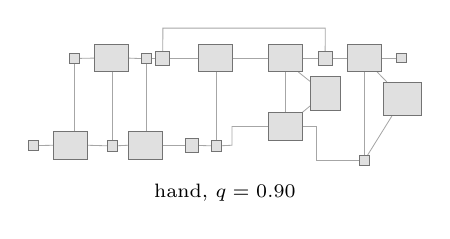
\begin{tikzpicture}[x=1cm,y=1cm,line width=0.3pt]
\draw[gray!70] (0.586,1.354) -- (0.842,1.359);
\draw[gray!70] (0.586,0.425) -- (0.586,1.354);
\draw[gray!70] (3.581,1.063) -- (3.429,1.185);
\draw[gray!70] (2.600,1.359) -- (3.056,1.359);
\draw[gray!70] (3.490,1.359) -- (3.772,1.359);
\draw[gray!70] (3.273,0.664) -- (3.273,1.185);
\draw[gray!70] (3.477,0.664) -- (3.581,0.751);
\draw[gray!70] (1.710,1.359) -- (2.166,1.359);
\draw[gray!70] (3.772,1.359) -- (3.774,1.740) -- (1.712,1.740) -- (1.710,1.359);
\draw[gray!70] (1.502,1.350) -- (1.710,1.359);
\draw[gray!70] (2.391,1.185) -- (2.391,0.243);
\draw[gray!70] (3.772,1.359) -- (4.054,1.359);
\draw[gray!70] (4.488,1.359) -- (4.744,1.359);
\draw[gray!70] (4.431,1.185) -- (4.557,1.055);
\draw[gray!70] (4.271,1.185) -- (4.271,0.061);
\draw[gray!70] (4.627,0.634) -- (4.271,0.061);
\draw[gray!70] (1.276,1.359) -- (1.502,1.350);
\draw[gray!70] (1.068,1.185) -- (1.068,0.243);
\draw[gray!70] (1.502,0.425) -- (1.502,1.350);
\draw[gray!70] (0.065,0.247) -- (0.321,0.252);
\draw[gray!70] (0.755,0.252) -- (1.068,0.243);
\draw[gray!70] (1.068,0.243) -- (1.276,0.252);
\draw[gray!70] (1.710,0.252) -- (2.079,0.252);
\draw[gray!70] (2.391,0.243) -- (2.589,0.252) -- (2.589,0.490) -- (3.056,0.490);
\draw[gray!70] (2.079,0.252) -- (2.391,0.243);
\draw[gray!70] (3.490,0.490) -- (3.659,0.490) -- (3.659,0.061) -- (4.271,0.061);
\draw[fill=black!12,draw=black!55] (0.521,1.289) rectangle (0.651,1.419);
\draw[fill=black!12,draw=black!55] (3.056,1.185) rectangle (3.490,1.532);
\draw[fill=black!12,draw=black!55] (3.581,0.699) rectangle (3.963,1.120);
\draw[fill=black!12,draw=black!55] (1.623,1.272) rectangle (1.797,1.445);
\draw[fill=black!12,draw=black!55] (2.166,1.185) rectangle (2.600,1.532);
\draw[fill=black!12,draw=black!55] (3.685,1.272) rectangle (3.859,1.445);
\draw[fill=black!12,draw=black!55] (4.054,1.185) rectangle (4.488,1.532);
\draw[fill=black!12,draw=black!55] (4.683,1.298) rectangle (4.805,1.419);
\draw[fill=black!12,draw=black!55] (4.514,0.634) rectangle (5.000,1.055);
\draw[fill=black!12,draw=black!55] (0.842,1.185) rectangle (1.276,1.532);
\draw[fill=black!12,draw=black!55] (1.437,1.285) rectangle (1.567,1.415);
\draw[fill=black!12,draw=black!55] (0.000,0.182) rectangle (0.130,0.312);
\draw[fill=black!12,draw=black!55] (0.321,0.078) rectangle (0.755,0.425);
\draw[fill=black!12,draw=black!55] (1.003,0.178) rectangle (1.133,0.308);
\draw[fill=black!12,draw=black!55] (1.276,0.078) rectangle (1.710,0.425);
\draw[fill=black!12,draw=black!55] (2.326,0.178) rectangle (2.457,0.308);
\draw[fill=black!12,draw=black!55] (3.056,0.317) rectangle (3.490,0.664);
\draw[fill=black!12,draw=black!55] (1.992,0.165) rectangle (2.166,0.339);
\draw[fill=black!12,draw=black!55] (4.210,0.000) rectangle (4.332,0.122);
\node[anchor=north,font=\scriptsize] at (2.50,-0.12) {hand, $q=0.90$};
\end{tikzpicture}
&
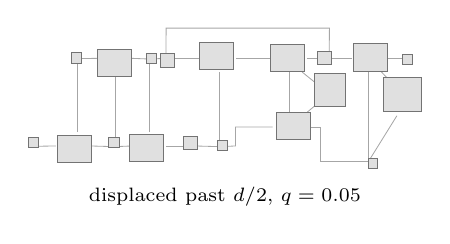
\begin{tikzpicture}[x=1cm,y=1cm,line width=0.3pt]
\draw[gray!70] (0.621,1.389) -- (0.878,1.393);
\draw[gray!70] (0.621,0.455) -- (0.621,1.389);
\draw[gray!70] (3.632,1.096) -- (3.480,1.219);
\draw[gray!70] (2.646,1.393) -- (3.104,1.393);
\draw[gray!70] (3.541,1.393) -- (3.824,1.393);
\draw[gray!70] (3.322,0.695) -- (3.322,1.219);
\draw[gray!70] (3.528,0.695) -- (3.632,0.782);
\draw[gray!70] (1.751,1.393) -- (2.209,1.393);
\draw[gray!70] (3.824,1.393) -- (3.827,1.777) -- (1.753,1.777) -- (1.751,1.393);
\draw[gray!70] (1.542,1.384) -- (1.751,1.393);
\draw[gray!70] (2.436,1.219) -- (2.436,0.271);
\draw[gray!70] (3.824,1.393) -- (4.108,1.393);
\draw[gray!70] (4.545,1.393) -- (4.802,1.393);
\draw[gray!70] (4.488,1.219) -- (4.614,1.088);
\draw[gray!70] (4.326,1.219) -- (4.326,0.088);
\draw[gray!70] (4.684,0.664) -- (4.326,0.088);
\draw[gray!70] (1.315,1.393) -- (1.542,1.384);
\draw[gray!70] (1.105,1.219) -- (1.105,0.271);
\draw[gray!70] (1.542,0.455) -- (1.542,1.384);
\draw[gray!70] (0.097,0.276) -- (0.354,0.280);
\draw[gray!70] (0.791,0.280) -- (1.105,0.271);
\draw[gray!70] (1.105,0.271) -- (1.315,0.280);
\draw[gray!70] (1.751,0.280) -- (2.122,0.280);
\draw[gray!70] (2.436,0.271) -- (2.635,0.280) -- (2.635,0.520) -- (3.104,0.520);
\draw[gray!70] (2.122,0.280) -- (2.436,0.271);
\draw[gray!70] (3.541,0.520) -- (3.711,0.520) -- (3.711,0.088) -- (4.326,0.088);
\draw[fill=black!12,draw=black!55] (0.546,1.332) rectangle (0.677,1.463);
\draw[fill=black!12,draw=black!55] (3.072,1.221) rectangle (3.509,1.570);
\draw[fill=black!12,draw=black!55] (3.642,0.782) rectangle (4.026,1.205);
\draw[fill=black!12,draw=black!55] (1.685,1.278) rectangle (1.859,1.453);
\draw[fill=black!12,draw=black!55] (2.170,1.251) rectangle (2.606,1.601);
\draw[fill=black!12,draw=black!55] (3.677,1.310) rectangle (3.851,1.484);
\draw[fill=black!12,draw=black!55] (4.131,1.230) rectangle (4.568,1.579);
\draw[fill=black!12,draw=black!55] (4.753,1.318) rectangle (4.875,1.440);
\draw[fill=black!12,draw=black!55] (4.511,0.723) rectangle (5.000,1.146);
\draw[fill=black!12,draw=black!55] (0.879,1.163) rectangle (1.316,1.512);
\draw[fill=black!12,draw=black!55] (1.503,1.326) rectangle (1.634,1.457);
\draw[fill=black!12,draw=black!55] (0.000,0.258) rectangle (0.131,0.389);
\draw[fill=black!12,draw=black!55] (0.374,0.071) rectangle (0.810,0.420);
\draw[fill=black!12,draw=black!55] (1.026,0.260) rectangle (1.157,0.391);
\draw[fill=black!12,draw=black!55] (1.286,0.078) rectangle (1.722,0.428);
\draw[fill=black!12,draw=black!55] (2.406,0.219) rectangle (2.537,0.350);
\draw[fill=black!12,draw=black!55] (3.155,0.360) rectangle (3.591,0.709);
\draw[fill=black!12,draw=black!55] (1.973,0.231) rectangle (2.147,0.406);
\draw[fill=black!12,draw=black!55] (4.316,0.000) rectangle (4.439,0.122);
\node[anchor=north,font=\scriptsize] at (2.50,-0.12) {displaced past $d/2$, $q=0.05$};
\end{tikzpicture}
&
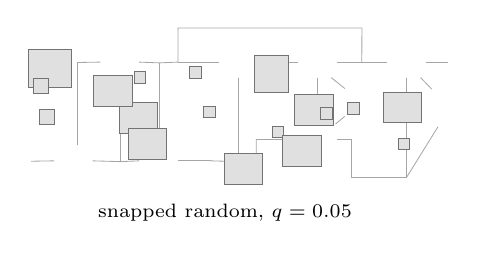
\begin{tikzpicture}[x=1cm,y=1cm,line width=0.3pt]
\draw[gray!70] (0.629,1.549) -- (0.919,1.554);
\draw[gray!70] (0.629,0.497) -- (0.629,1.549);
\draw[gray!70] (4.022,1.219) -- (3.850,1.357);
\draw[gray!70] (2.911,1.554) -- (3.427,1.554);
\draw[gray!70] (3.918,1.554) -- (4.238,1.554);
\draw[gray!70] (3.673,0.767) -- (3.673,1.357);
\draw[gray!70] (3.904,0.767) -- (4.022,0.865);
\draw[gray!70] (1.903,1.554) -- (2.419,1.554);
\draw[gray!70] (4.238,1.554) -- (4.240,1.986) -- (1.905,1.986) -- (1.903,1.554);
\draw[gray!70] (1.667,1.544) -- (1.903,1.554);
\draw[gray!70] (2.675,1.357) -- (2.675,0.290);
\draw[gray!70] (4.238,1.554) -- (4.558,1.554);
\draw[gray!70] (5.049,1.554) -- (5.339,1.554);
\draw[gray!70] (4.985,1.357) -- (5.128,1.209);
\draw[gray!70] (4.803,1.357) -- (4.803,0.084);
\draw[gray!70] (5.206,0.733) -- (4.803,0.084);
\draw[gray!70] (1.411,1.554) -- (1.667,1.544);
\draw[gray!70] (1.175,1.357) -- (1.175,0.290);
\draw[gray!70] (1.667,0.497) -- (1.667,1.544);
\draw[gray!70] (0.039,0.295) -- (0.329,0.300);
\draw[gray!70] (0.821,0.300) -- (1.175,0.290);
\draw[gray!70] (1.175,0.290) -- (1.411,0.300);
\draw[gray!70] (1.903,0.300) -- (2.321,0.300);
\draw[gray!70] (2.675,0.290) -- (2.898,0.300) -- (2.898,0.570) -- (3.427,0.570);
\draw[gray!70] (2.321,0.300) -- (2.675,0.290);
\draw[gray!70] (3.918,0.570) -- (4.110,0.570) -- (4.110,0.084) -- (4.803,0.084);
\draw[fill=black!12,draw=black!55] (2.232,0.846) rectangle (2.380,0.993);
\draw[fill=black!12,draw=black!55] (1.155,0.649) rectangle (1.647,1.042);
\draw[fill=black!12,draw=black!55] (2.871,1.163) rectangle (3.304,1.640);
\draw[fill=black!12,draw=black!55] (3.441,0.413) rectangle (3.638,0.610);
\draw[fill=black!12,draw=black!55] (0.831,0.993) rectangle (1.323,1.386);
\draw[fill=black!12,draw=black!55] (0.143,0.762) rectangle (0.339,0.959);
\draw[fill=black!12,draw=black!55] (3.382,0.752) rectangle (3.874,1.146);
\draw[fill=black!12,draw=black!55] (3.102,0.595) rectangle (3.240,0.733);
\draw[fill=black!12,draw=black!55] (0.000,1.236) rectangle (0.551,1.713);
\draw[fill=black!12,draw=black!55] (2.488,0.000) rectangle (2.979,0.393);
\draw[fill=black!12,draw=black!55] (3.717,0.826) rectangle (3.864,0.973);
\draw[fill=black!12,draw=black!55] (1.347,1.288) rectangle (1.495,1.436);
\draw[fill=black!12,draw=black!55] (3.230,0.231) rectangle (3.722,0.624);
\draw[fill=black!12,draw=black!55] (2.055,1.352) rectangle (2.203,1.500);
\draw[fill=black!12,draw=black!55] (1.268,0.320) rectangle (1.760,0.713);
\draw[fill=black!12,draw=black!55] (4.061,0.890) rectangle (4.208,1.037);
\draw[fill=black!12,draw=black!55] (4.508,0.782) rectangle (5.000,1.175);
\draw[fill=black!12,draw=black!55] (0.064,1.155) rectangle (0.261,1.352);
\draw[fill=black!12,draw=black!55] (4.700,0.447) rectangle (4.838,0.585);
\node[anchor=north,font=\scriptsize] at (2.50,-0.12) {snapped random, $q=0.05$};
\end{tikzpicture}
\end{tabular}
\caption{The alignment controls on one BPMN model (19 boxes; the corpus medians are
$0.91$, $0.20$ and $0.07$). Left, the drawing as its author left it. Centre, every box
displaced by up to 15 units, just past the $d/2$ below which the directional test cannot
resolve a misalignment. Right, every box placed uniformly at random in the same bounding
box and snapped to the same grid: the grid is available and the author is not. Box sizes
are unchanged throughout; edges are the routes the file stores.}
\label{fig:controls}
\end{figure}


The rest, each with the test that excluded it and the numbers it turned on:

\begin{center}\small
\begin{tabular}{@{}p{2.5cm}p{4.1cm}p{7.7cm}@{}}
\toprule
alternative & test & result \\
\midrule
Reference length
 & $L$ at the median edge length and at $1/\sqrt{N}$
 & hand held on 0.00 to 0.06 of boxes under length and stress, as under the fit; only the
   control moves \\[2pt]
Straight segments where the person drew polylines
 & primary tables on the stored routes, chords beside them
 & no verdict moves \\[2pt]
A constrained energy whose constraints are absent
 & the flow term in the tables; the BPMN lanes decomposed
 & flow holds 0.59 to 0.85 of hand-placed boxes, so reading direction is a criterion partly
   satisfied and not the missing constraint; 43\% of held BPMN boxes are held by an
   alignment no horizontal lane can impose, and the lanes of the rest leave a median 6.3
   box heights of room. Containment as a hard constraint was not added \\[2pt]
The radius
 & $d \in \{0.005, 0.01, 0.02, 0.05\}$; at $d=0.02$ the move is about one grid step
 & the hand verdicts are the same at every $d$. The table at $d$ in units of box width and
   of median edge length was not run \\[2pt]
Selection: near-trees make overlap and crossings easy
 & $q$ against $m/n$ over diagrams (\texttt{sparsity.py})
 & crossings do track density (Spearman $\rho$ $-0.37$, $-0.34$, $-0.11$ by hand and
   $-0.48$, $-0.30$, $-0.41$ for \texttt{dot}), these being near-trees at $m/n$ 1.06, 1.04
   and 1.11 against 1.30 in the Rome benchmark \cite{rome}, so ``crossings hold every box''
   is partly the trees' gift, given to every layout of the same graphs alike; crossings are
   what the theory is about \cite{gj83}, and on these diagrams there are few to remove. Overlap does
   not ($+0.02$, $-0.06$, $+0.12$), and length and stress are 0.00 in the sparse and the
   dense half both. No hand--tool difference is explained \\[2pt]
The tools are the wrong tools
 & ELK layered 0.12.0, the engine the BPMN and KIELER editors run, as a fourth control
 & its profile is \texttt{dot}'s: length and stress 0.00, flow 1.00 at value 0.000,
   alignment 0.42 to 0.62 where \texttt{dot} reaches 0.89 to 1.00 \\
\bottomrule
\end{tabular}
\end{center}

\section{The pre-registration's scorecard}\label{app:prereg}

An earlier version of this study took 147 BPMN models without the connector filter,
two fifths of them read as bipartite graphs.

The registered $d$ = one grid pitch (\texttt{results/pitch.md}), 0.0008 to 0.0017 of
the width per diagram: hand length and stress hold 0.00 with 0.99 to 1.00 of diagrams
exactly there, A1 keeps its gap (0.11 and 0.83 against \texttt{neato}'s 0.00 and 0.04),
and \texttt{neato}'s stress at 0.76 and 0.80 extends the radius sweep's left edge.
WikiPathways has no detected pitch, out of scope as registered.

\paragraph{The pre-registration's scorecard.} H1, crossings and overlap hold the hand
layout above 0.9 and above \texttt{neato}: holds, 1.00 against 0.41 to 0.76. H2, length
alone holds under 0.2 and below \texttt{neato}: holds, 0.00 against 0.24 to 0.42. H3, no
positive length weight repairs $C{+}O{+}L$: holds, fitted weight 0.000 everywhere and $q$
0.008 at any weight past 0.001. H4, alignment holds more boxes than orthogonality or
node--edge in every corpus: \textbf{refuted}. Node--edge holds 0.88, 1.00 and 1.00 of
hand-placed boxes against alignment's 0.52, 0.21 and 0.91. Node--edge is priced in the
standard energy and alignment is not, so the omitted-term conclusion stands, but the
registered ranking was wrong and the recorded prediction with it. H5, exploratory, stress
holds the hand layout less than \texttt{neato}'s: holds, 0.00 against 1.00. The registered
fourth corpus, HOLA's formative drawings, was dropped undeclared from the previous draft;
it is restored above. The deduplication pass is run in Section~\ref{sec:corpora} and
the 41--100 band above. Registered and still not run: the caps in pitch units.

\section{Deduplication and drawers}\label{app:dedup}

194 of the 248 Reactome graphs and 120 of the 300 BPMN graphs in the band are the
component of a larger diagram; no WikiPathways pathway in the band is.

The 136 drawings are
17 participants crossed with 8 graphs, so the interval is clustered: resampling
participants (2000 draws) puts the alignment median at [0.31, 0.57], and the
per-participant medians run 0.14 to 0.96. Across the four corpora the seven terms every
corpus measures rank in the same order, Kendall's $W = 0.99$.

The registered deduplication pass
(\texttt{results/dedup.py}): by exact coordinate multiset, one Reactome pair is a single
drawing stored under two ids; by the structural key ($n$, $m$, degree sequence, box
sizes), one further Reactome pair and one WikiPathways pair; the 300 BPMN models collide
under neither key, so the feared resubmission duplicates are absent from this sample.
Removing every extra member moves no headline median. Clustering by drawer: the 305
WikiPathways pathways carry 153 first authors, the most prolific 9\% of the corpus; the
A1 median's interval clustered by first author is [0.48, 0.55] against [0.48, 0.54] over
diagrams, and the twenty drawers of three or more pathways hold medians 0.19 to 0.85
(\texttt{results/drawers.py}). Reactome curators and BPMN authors are not recorded in
the archives as parsed.

\section{Reproducibility}\label{app:repro}

Parsers, the energy, the test, the descent, the fitting scripts, the parsed corpora and
every table's script are in the repository under \texttt{example/diagrams}; the main
tables rebuild by \texttt{results/run\_all.sh}, and every sensitivity of the appendix
ships its script beside its committed output. \texttt{results/manifest.txt} records
commit, platform, tool versions, seeds and the SHA-256 of the archives and the corpora
as measured. The tracked \texttt{data/bpmn\_population\_a1.csv} rebuilds the abstract's
0.87 from a clone; the repository carries derived coordinates and ids, never archive
content, and the two biological corpora are CC-licensed exports.

\section{Related work, tabulated}\label{app:related}

\begin{center}\small
\begin{tabular}{@{}p{3.5cm}p{5.2cm}p{5.6cm}@{}}
\toprule
work & what it did & what it gives, and what it leaves \\
\midrule
\multicolumn{3}{@{}l}{\emph{By having people draw}}\\[2pt]
van Ham, Rogowitz \cite{vanham08}
 & 73 hand layouts against a force-directed algorithm, half started from its optimum
 & 71 of 73 raise edge-length variance above the optimum; 60\% fewer crossings \\[2pt]
Dwyer et al.\ \cite{dwyer09}
 & 32 participants laid out one graph; 194 judges ranked the results against three
   automatic layouts
 & judges' choices track stress, without a test; its Table 2 has user layouts at 3 to 9
   times the force-directed stress \\[2pt]
Purchase, Pilcher, Plimmer \cite{purchase12}
 & participants drew from adjacency lists
 & crossing removal the strongest aesthetic, alignment to a grid important \\[2pt]
Kieffer et al.\ \cite{hola16}
 & 17 participants' layouts of 8 small graphs, ranked by 66 judges
 & gridiness correlates with rank on all 8, the source of HOLA's alignment step; rank
   tracks stress on 4 of 8 \\[2pt]
Mooney et al.\ \cite{mooney25}
 & preference and shortest-path performance against stress, graphs to 50 nodes
 & people prefer low stress and perform better as it falls; why the conclusion adds a term
   and removes none \\[2pt]
Mooney et al.\ \cite{gdcoll25}
 & 4{,}890 drawings harvested automatically from 27 editions of these proceedings
 & measured in Section~\ref{sec:results}: length and stress 0.00, alignment 0.87.
   Provenance is not per drawing and edge directions are dropped, so flow and the box
   terms are not run \\[4pt]
\multicolumn{3}{@{}l}{\emph{By showing people drawings}}\\[2pt]
Purchase et al.\ \cite{purchase20}
 & a Turing test on hand and algorithmic drawings
 & hand drawings distinguishable, and judged better \\[2pt]
Klammler, Mchedlidze, Pak \cite{klammler19}
 & Nelder--Mead fit of a linear aesthetic combination discriminating good from worsened
   layouts
 & no human coordinates enter it; they call human-labelled data a critically important
   accomplishment still to come \\[4pt]
\multicolumn{3}{@{}l}{\emph{By learning from examples}}\\[2pt]
Masui \cite{masui94}
 & a weighted constraint combination from good and bad layouts, by genetic programming
 & neither tested whether the examples are minima of the learned energy \\[2pt]
Sp\"onemann et al.\ \cite{spoenemann14}
 & weights adjusted from user selections among candidates
 & as above \\[2pt]
Flud \cite{flud22}
 & annealing continued from crowd layouts of pathway diagrams, three networks
 & the closest prior descent from a hand layout; it raised an asserted five-term score and
   read that as success. The cap, the per-term test, the reference and the controls here
   are what make it a measurement of the score \\[2pt]
Zhang et al.\ \cite{zhang26}
 & 64{,}222 pairwise preference labels
 & the nearest recent work; it learns from preferences, not coordinates \\[2pt]
Wang et al.\ \cite{deepgd21}
 & a graph network drawing arbitrary graphs under a weighted sum of aesthetics
 & the weights are asserted or tuned, not learned from people; no human coordinates
   enter it \\[2pt]
O'Donovan, Agarwala, Hertzmann \cite{odonovan14}
 & a 122-parameter energy over single-page graphic designs fitted to a handful of human
   examples by nonlinear inverse optimisation
 & each example taken as optimal under the unknown parameters: the assumption examined
   here, and the closest prior instance of it we found \\
\bottomrule
\end{tabular}
\end{center}


\end{document}
